% Options for packages loaded elsewhere
\PassOptionsToPackage{unicode}{hyperref}
\PassOptionsToPackage{hyphens}{url}
\PassOptionsToPackage{dvipsnames,svgnames,x11names}{xcolor}
%
\documentclass[
default
]{sn-jnl}

\usepackage{amsmath,amssymb}
\usepackage{iftex}
\ifPDFTeX
  \usepackage[T1]{fontenc}
  \usepackage[utf8]{inputenc}
  \usepackage{textcomp} % provide euro and other symbols
\else % if luatex or xetex
  \usepackage{unicode-math}
  \defaultfontfeatures{Scale=MatchLowercase}
  \defaultfontfeatures[\rmfamily]{Ligatures=TeX,Scale=1}
\fi
\usepackage{lmodern}
\ifPDFTeX\else  
    % xetex/luatex font selection
\fi
% Use upquote if available, for straight quotes in verbatim environments
\IfFileExists{upquote.sty}{\usepackage{upquote}}{}
\IfFileExists{microtype.sty}{% use microtype if available
  \usepackage[]{microtype}
  \UseMicrotypeSet[protrusion]{basicmath} % disable protrusion for tt fonts
}{}
\makeatletter
\@ifundefined{KOMAClassName}{% if non-KOMA class
  \IfFileExists{parskip.sty}{%
    \usepackage{parskip}
  }{% else
    \setlength{\parindent}{0pt}
    \setlength{\parskip}{6pt plus 2pt minus 1pt}}
}{% if KOMA class
  \KOMAoptions{parskip=half}}
\makeatother
\usepackage{xcolor}
\setlength{\emergencystretch}{3em} % prevent overfull lines
\setcounter{secnumdepth}{-\maxdimen} % remove section numbering
% Make \paragraph and \subparagraph free-standing
\ifx\paragraph\undefined\else
  \let\oldparagraph\paragraph
  \renewcommand{\paragraph}[1]{\oldparagraph{#1}\mbox{}}
\fi
\ifx\subparagraph\undefined\else
  \let\oldsubparagraph\subparagraph
  \renewcommand{\subparagraph}[1]{\oldsubparagraph{#1}\mbox{}}
\fi


\providecommand{\tightlist}{%
  \setlength{\itemsep}{0pt}\setlength{\parskip}{0pt}}\usepackage{longtable,booktabs,array}
\usepackage{calc} % for calculating minipage widths
% Correct order of tables after \paragraph or \subparagraph
\usepackage{etoolbox}
\makeatletter
\patchcmd\longtable{\par}{\if@noskipsec\mbox{}\fi\par}{}{}
\makeatother
% Allow footnotes in longtable head/foot
\IfFileExists{footnotehyper.sty}{\usepackage{footnotehyper}}{\usepackage{footnote}}
\makesavenoteenv{longtable}
\usepackage{graphicx}
\makeatletter
\def\maxwidth{\ifdim\Gin@nat@width>\linewidth\linewidth\else\Gin@nat@width\fi}
\def\maxheight{\ifdim\Gin@nat@height>\textheight\textheight\else\Gin@nat@height\fi}
\makeatother
% Scale images if necessary, so that they will not overflow the page
% margins by default, and it is still possible to overwrite the defaults
% using explicit options in \includegraphics[width, height, ...]{}
\setkeys{Gin}{width=\maxwidth,height=\maxheight,keepaspectratio}
% Set default figure placement to htbp
\makeatletter
\def\fps@figure{htbp}
\makeatother
% definitions for citeproc citations
\NewDocumentCommand\citeproctext{}{}
\NewDocumentCommand\citeproc{mm}{%
  \begingroup\def\citeproctext{#2}\cite{#1}\endgroup}
\makeatletter
 % allow citations to break across lines
 \let\@cite@ofmt\@firstofone
 % avoid brackets around text for \cite:
 \def\@biblabel#1{}
 \def\@cite#1#2{{#1\if@tempswa , #2\fi}}
\makeatother
\newlength{\cslhangindent}
\setlength{\cslhangindent}{1.5em}
\newlength{\csllabelwidth}
\setlength{\csllabelwidth}{3em}
\newenvironment{CSLReferences}[2] % #1 hanging-indent, #2 entry-spacing
 {\begin{list}{}{%
  \setlength{\itemindent}{0pt}
  \setlength{\leftmargin}{0pt}
  \setlength{\parsep}{0pt}
  % turn on hanging indent if param 1 is 1
  \ifodd #1
   \setlength{\leftmargin}{\cslhangindent}
   \setlength{\itemindent}{-1\cslhangindent}
  \fi
  % set entry spacing
  \setlength{\itemsep}{#2\baselineskip}}}
 {\end{list}}
\usepackage{calc}
\newcommand{\CSLBlock}[1]{\hfill\break\parbox[t]{\linewidth}{\strut\ignorespaces#1\strut}}
\newcommand{\CSLLeftMargin}[1]{\parbox[t]{\csllabelwidth}{\strut#1\strut}}
\newcommand{\CSLRightInline}[1]{\parbox[t]{\linewidth - \csllabelwidth}{\strut#1\strut}}
\newcommand{\CSLIndent}[1]{\hspace{\cslhangindent}#1}

%%%% Standard Packages

\usepackage{graphicx}%
\usepackage{multirow}%
\usepackage{amsmath,amssymb,amsfonts}%
\usepackage{amsthm}%
\usepackage{mathrsfs}%
\usepackage[title]{appendix}%
\usepackage{xcolor}%
\usepackage{textcomp}%
\usepackage{manyfoot}%
\usepackage{booktabs}%
\usepackage{algorithm}%
\usepackage{algorithmicx}%
\usepackage{algpseudocode}%
\usepackage{listings}%

%%%%

\raggedbottom
\usepackage{fontspec}
\usepackage{multirow}
\usepackage{multicol}
\usepackage{colortbl}
\usepackage{hhline}
\newlength\Oldarrayrulewidth
\newlength\Oldtabcolsep
\usepackage{longtable}
\usepackage{array}
\usepackage{hyperref}
\usepackage{float}
\usepackage{wrapfig}
\makeatletter
\@ifpackageloaded{caption}{}{\usepackage{caption}}
\AtBeginDocument{%
\ifdefined\contentsname
  \renewcommand*\contentsname{Table of contents}
\else
  \newcommand\contentsname{Table of contents}
\fi
\ifdefined\listfigurename
  \renewcommand*\listfigurename{List of Figures}
\else
  \newcommand\listfigurename{List of Figures}
\fi
\ifdefined\listtablename
  \renewcommand*\listtablename{List of Tables}
\else
  \newcommand\listtablename{List of Tables}
\fi
\ifdefined\figurename
  \renewcommand*\figurename{Figure}
\else
  \newcommand\figurename{Figure}
\fi
\ifdefined\tablename
  \renewcommand*\tablename{Table}
\else
  \newcommand\tablename{Table}
\fi
}
\@ifpackageloaded{float}{}{\usepackage{float}}
\floatstyle{ruled}
\@ifundefined{c@chapter}{\newfloat{codelisting}{h}{lop}}{\newfloat{codelisting}{h}{lop}[chapter]}
\floatname{codelisting}{Listing}
\newcommand*\listoflistings{\listof{codelisting}{List of Listings}}
\makeatother
\makeatletter
\makeatother
\makeatletter
\@ifpackageloaded{caption}{}{\usepackage{caption}}
\@ifpackageloaded{subcaption}{}{\usepackage{subcaption}}
\makeatother
\ifLuaTeX
  \usepackage{selnolig}  % disable illegal ligatures
\fi
\usepackage{bookmark}

\IfFileExists{xurl.sty}{\usepackage{xurl}}{} % add URL line breaks if available
\urlstyle{same} % disable monospaced font for URLs
\hypersetup{
  pdftitle={School closures and consolidations: the active travel and emission implications of reduced accessibility},
  pdfauthor={Anastasia Soukhov; Christopher D. Higgins; Antonio Páez; Moataz Mohamed},
  pdfkeywords={accessibility; spatial availability; carbon emissions;
journey-to-school; walkability; active transportation; school
consolidation policy; service provision thresholds},
  colorlinks=true,
  linkcolor={blue},
  filecolor={Maroon},
  citecolor={Blue},
  urlcolor={Blue},
  pdfcreator={LaTeX via pandoc}}

\title[School closures and consolidations: the active travel and
emission implications of reduced accessibility]{School closures and
consolidations: the active travel and emission implications of reduced
accessibility}

% author setup
\author*[1]{\fnm{Anastasia} \sur{Soukhov}}\email{soukhoa@mcmaster.ca}\author[2]{\fnm{Christopher D.} \sur{Higgins}}\email{cd.higgins@utoronto.ca}\author[1]{\fnm{Antonio} \sur{Páez}}\email{paezha@mcmaster.ca}\author[3]{\fnm{Moataz} \sur{Mohamed}}\email{mmohame@mcmaster.ca}
% affil setup
\affil[1]{, \orgaddress{\street{School of Earth, Environment and
Society, McMaster University, 1241 Main St.~West, Hamilton, ON, L8S 4K1,
Canada}}}
\affil[2]{, \orgaddress{\street{Department of Human Geography,
University of Toronto Scarborough, 1265 Military Trail, Toronto, ON, M1C
1A4, Canada}}}
\affil[3]{, \orgaddress{\street{Department of Civil Engineering,
McMaster University, 1241 Main St.~West, Hamilton, ON, L8S 4K1,
Canada}}}

% abstract 

\abstract{Reducing emissions and increasing active travel are top
priorities for many communities. Often, though, these priorities are
confronted with pressures to reduce the fiscal burden of public
services, including schools. Public schools have been strained to do
more with less, and governments are opting to close under-capacity
schools and expand existing schools to accommodate lost capacity. The
objective of this study is to quantify the travel burdens of school
consolidation/closure policies. We do this through the case of Hamilton,
a mid-sized city in Ontario, Canada. Between the years 2011 and 2015,
7\% of the elementary schools closed in the city. We study how these
closures changed the accessibility landscape for the elementary school
aged population, as well as the active travel and emission implications.
In terms of methods, we use spatial availability, a singly-constrained
multimodal measure of spatial accessibility. Thanks to its proportional
allocation mechanism, spatial availability allows for an interpretable
comparison between `before' and `after' the implementation of school
closure/consolidation policy. Analysis is conducted at the parcel-level
with all school seats being eligible and travel behaviour based on
observed home-to-school patterns for motorized and non-motorized modes.
We report estimates of system-wide impacts that result from the
closures, such as potential growth in GHG emission and reduction of
walking minutes. Findings demonstrate that overall, spatial availability
decreased in the city. Though the school consolidation policy may have
resulted in cost-savings in operation and maintenance of facilities,
students, families, and communities pay the price in reduced
opportunities for physical activity and greater motorized
mobility-related pollution.}

% keywords
\keywords{accessibility; spatial availability; carbon emissions;
journey-to-school; walkability; active transportation; school
consolidation policy; service provision thresholds}

\begin{document}
\maketitle

\section{Introduction}\label{introduction}

Communities are by nature in flux: economic and demographic shifts,
rural and urban configurations, and political pressures all combine to
produce change. These forces spur the re-organization and consolidation
of public facilities in communities around the world where changes to
service provision may improve the quality of service for some but not
for all (Christiaanse 2020; Rosik, Puławska-Obiedowska, and Goliszek
2021). While change is natural, oftentimes top-down consolidation
decisions are driven by operational cost-savings that do not take into
consideration the full extent of losses in benefits.

From this perspective, school closure policies have been pursued by
governments to optimize per-student operational cost-efficiency (Rong et
al. 2022; Dai et al. 2019) but other implications, such as the impact of
closures on property values (Merrall, Higgins, and Páez 2024), their
effects on the social infrastructure of communities (Butler, Kane, and
Cooligan 2019; Irwin and Seasons 2012), and particularly their travel
implications have often been overlooked by decision makers (Bierbaum,
Karner, and Barajas 2021; J. Lee and Lubienski 2017). This seems a
mistake: journey-to-school trips are tremendously important, and travel
for this purpose is currently the largest contributor of carbon
emissions from personal travel after the journey-to-work (Rong et al.
2022; Pantelaki, Claudia Caspani, and Maggi 2024), where it could be
instead an excellent opportunity for physical activity (Desjardins et
al. 2024). Alas, in many communities globally, schools are closing
(Sageman 2022). For instance, 65\% of comprehensive schools (e.g.~grades
1 through 9) in rural Finland since 1990 closed (Autti and
Hyry-Beihammer 2014), 10\% of elementary schools (kindergarten through
grade 8) in Chicago, USA in 2013 (J. Lee and Lubienski 2017), and 7\% of
primary and lower secondary schools (kindergarten through grade 9) were
closed in Denmark between 2010-2011 (Beuchert et al. 2018). School
closures often increase the distance to school for many students and
thus tend to induce motorized trips (Rong et al. 2022).

We focus on the transportation implications of school closure and
consolidation policies. While some research has considered the ``steps
in reserve'', that is, the potential for active travel hidden behind
motorized trips (Morency, Roorda, and Demers 2009; Morency, Demers, and
Lapierre 2007), school closures potentially make actual steps vanish,
sent to the reserve for the foreseeable future. In exchange for less
physical activity, communities get more motorized travel, with the
concomitant costs and burdens, including emissions. Quantification of
losses in potential active travel and associated growth in carbon
emissions is scarce in the literature, and the focus of this paper. In
addition to its empirical contributions, this work makes use of a novel
multimodal and singly-constrained accessibility measure, called spatial
availability (Soukhov et al. 2023; Soukhov et al. 2024), which we use to
estimate the changes in accessibility and travel after a recent wave of
school closures/consolidations in Hamilton, Ontario.

The results of the research indicate that, overall, school seats became
less spatially available in the city. This change happened unevenly,
with some communities being disproportionately affected. Though the
school consolidation policy pursued by the province and implemented by
the local school board may have resulted in cost-savings in operation
and maintenance of facilities, families, students, and communities now
pay the price in terms of lost opportunities for healthier active
travel, as well as increased emissions from motorized travel.

\section{Background}\label{background}

Hamilton is a mid-size city (\textasciitilde570,000 pop) with rural,
suburban and urban characteristics in the province of Ontario, Canada
(Government of Canada 2022). In 2013, the Hamilton-Wentworth District
School Board (HWDSB), the largest public English school board in the
city, released its Long Term Facilities Master Plan (HWDSB 2013). To
ensure ``equitable, affordable and sustainable learning facilities'',
the Master Plan indicated that 80\% of its elementary schools (attended
by students aged 5 to 13) would be subjected to accommodation
evaluations, including an ``Accommodation Review'', the outcome of which
historically has been school closures/consolidations (HWDSB 2013; Craggs
2013; Seasons 2014b). These decisions, underhandedly supported by the
province, were in part motivated by a search for operational savings
based on projected reductions in student population and underutilized
school capacity (Craggs 2012). Hamilton was particularly affected, as
the HWDSB underwent an unprecedented number of Accommodation Reviews
relative to other school boards (Seasons 2014a).

Though the Accommodation Review guidelines outline a community-focused
process to assess the value that a school provides to students, the
community, and the local economy (Seasons 2014b; Ministry of Education
2006), in practice residents felt that a wholesome breakdown of costs to
repair/maintain schools was not made consistently available (Kleinhuis
2013). Further, others pointed to flawed incentive structures motivating
the HWDSB: ``By closing three schools the HWDSB would have a strong case
with the Ministry of Education to receive full funding for a new
school'' (Kleinhuis 2013). Along with insufficient funding to maintain
schools in a state of good repair (Auditor General of Ontario 2015), the
operational savings as a case for school closures is a long-standing
critique of the school ``funding formula'' established by the
conservative provincial government in 1998 (Mackenzie 2018; Irwin and
Seasons 2012). Within a backdrop of budget cuts, the funding formula
pits the financing of school maintenance and student needs against the
financial compensation of staff and the powers of local school boards,
which depend on the province for the allocation of resources (Mackenzie
2018).

In the wave of school accommodation reviews between 2013 and 2016, 12
elementary schools closed in Hamilton. These closures represented a 7\%
and 4\% decline in elementary school locations and capacity between 2011
(before the school closures) and 2016, despite the elementary-aged
student population in the city slightly increasing between 2011 and
2016( from 58,265 students to 58,865 students).

While accommodation reviews were undertaken to reduce operational costs,
how might have the closure of schools impacted local communities? In
this paper, we hypothesize that the school consolidation policy reduced
accessibility to schools for many students. By extension, this loss in
access and the consequent displacement of active trips to school
increased transportation-related emissions. To test these hypotheses,
the paper examines the following: how does the (1) spatial availability,
(2) loss in walk minutes and (3) associated carbon emissions change for
home-to-school trips after a city closes and consolidates schools?
Further, this work examines (4) what communities, based on low-income
prevalence, experienced the greatest losses as a result of this policy.

Spatial availability, a singly-constrained measure of spatial
accessibility (Soukhov et al. 2023; Soukhov et al. 2024), is used to
quantify accessibility before- and after- school closures, and the
associated impacts for the city of Hamilton and the elementary
school-aged student population as a result of a policy with narrowly
defined benefits. The methods used in this paper can be applied by
decision-makers to evaluate the spatial and transport-related impacts of
public service provision policy. Furthermore, to increase the diffusion
of this analysis, all work is transparent and reproducible, following
best practices in the spatial sciences (Brunsdon and Comber 2021;
Antonio Páez 2021). Accordingly, all associated code and data will be
publicly available within the lead author's
\href{https://github.com/soukhova/School-closures-accessibility-impacts}{GitHub
repository}

\section{Data}\label{data}

Our focus is to evaluate the impact of school consolidations between
2011 and 2016 on multimodal school spatial availability and
travel-related GHG emission in Hamilton. To facilitate comparison, two
scenarios are generated. Each scenario reflects the conditions in 2011
and 2016 respectively, assuming the school configurations in each year,
as well as average student population and low-income prevalence of
households, residential parcel locations, and estimated modal travel
times. The difference between the two scenarios is quantified in terms
of accessibility, emissions and equity implications and discussed in
context with the school consolidation policy. Data was retrieved at
different levels of spatial granularity from the following sources.

\subsection{Schools}\label{schools}

First, schools and associated school catchments were retrieved from the
City's school boards. In Hamilton, the majority of student-aged
population attends a school in one of the two English public school
boards (FAO 2023). One board is referred to as \emph{public} (i.e.,
Hamilton Wentworth District School Board (HWDSB)) in our work and the
other is referred to as \emph{public-catholic} (Hamilton Wentworth
Catholic District School Board (HWCDSB)). These catchments indicate what
residential property is assigned to what school, by default. Families
can decide to attend schools out of catchment; in fact, 21\%-23\% of
motorized school trips are out of catchment according to the regional
travel survey, the Transportation Tomorrow Survey (TTS) in 2011 and 2016
(Data Management Group 2018). The elementary school locations and
catchments were provided by the HWDSB and HWCDSB for the 2010-2011 and
2015-2016 academic years, and are shown in Figure~\ref{fig-Fig1}.

Formally, elementary schools are defined as schools that provide
instruction to any combination of grades between kindergarten to grade 8
(i.e.~typically children aged 5 to 14). As such, elementary includes
middle schools that only instruct grades 6 to 8 (\emph{MidElem}),
primary schools that only instruct kindergarten to grade 5 or 6
(\emph{JrElem}), and all grade elementary schools (\emph{Elem}) which
instruct all grades from kindergarten to grade 8. The number of `seats'
available in the school beyond or below which it will be over/under-
capacity is calculated by the provincial Ministry of Education; this
value is referred to as the on-the-ground capacity (\emph{OTGC}), and is
assigned to each school. The current/historic OTGCs are not publicly
available (Ontario 2017). However, for schools that underwent the full
Accommodation Review process, OTGCs for a given year could be obtained
from publicly available School Information Profiles. A regression model
was used to estimate the OTGCs for schools that lacked OTGC information.
The independent variables in the model were 1) the school's building
footprint (\emph{F}) in units of (\(m^2\)); 2) the school's shortest
Euclidean distance from the centroid of Hamilton's central business
district area (\emph{DistCBD}) defined in units of (m); and 3)
coefficients associated with a binary variable indicating the type of
school grade instruction (\emph{MidElem}, \emph{JrElem}, \emph{Elem}).
The building footprint from an archived spatial data set (Spatial 2015)
and the 2016 footprints were retrieved from OSM (OpenStreetMap 2021).
Because the age of construction for different schools is not available,
we used each school's distance from the centroid of the Downtown
Business Improvement Area (Hamilton 2014) as a proxy for school age as
the oldest buildings are generally located closer to the city centre
(Merrall 2021). Of note, the models were also used to estimate OTGC of
secondary schools (\emph{Sec}) though not included in the scope of this
work; these public institutions provide instruction for grades 9 to 12
(i.e., children aged 14 to 17).

Equations (\ref{eq:OTGC-public}) and (\ref{eq:OTGC-catholic}) describe
the estimated OTGC for public schools and catholic schools respectively.
School status and OTGC summed by catchment is also visualised in
Figure~\ref{fig-Fig1}. As seen in Table \ref{TabA1-OTGC} in the
Appendix, the coefficient of determination for these models is
\(R^2 = 0.999\) and \(R^2 = 0.998\) for the Public \(OTGC_{Public}\) and
Catholic \(OTGC_{Catholic}\) Boards respectively, and the residual
standard deviation is \(\sigma = 0.212\) and \(sigma = 0.331\).

\begin{equation}
\label{eq:OTGC-public}
OTGC_{Public} = F^{0.346}-e^{0.00003*DistCBD}+e^{3.123*JrElem}+e^{3.752*Elem}+ e^{3.068*MidElem} 
\end{equation}

\begin{equation}
\label{eq:OTGC-catholic}
OTGC_{Catholic} =F^{0.471}-e^{0.00003*DistCBD}+e^{2.333*Elem}
\end{equation}

\begin{figure}

\centering{

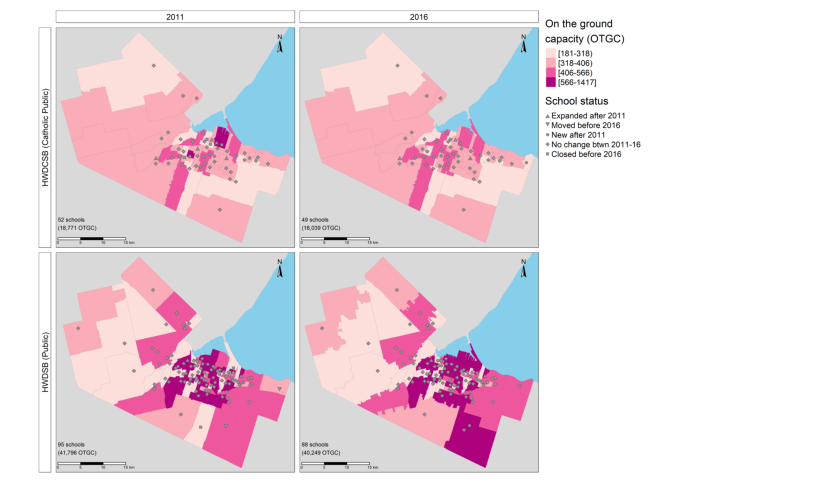
\includegraphics[width=1.2\textwidth,height=\textheight]{Manuscript_files/figure-pdf/fig-Fig1-1.pdf}

}

\caption{\label{fig-Fig1}The school catchments, estimated On The Ground
Capacity (OTGC) of schools summed per catchment, and school status for
both public and public catholic school boards for year 2011 and 2016.
OTGC scale is presented by quartiles.}

\end{figure}%

\subsection{Students, residential locations and low-income
prevelance}\label{students-residential-locations-and-low-income-prevelance}

In addition to OTGC for schools, statistics about the student population
and proportion of low-income after tax (LIM-AT) households were
retrieved from the 2011 and 2016 Canadian Census (Canada 2011, 2016)
using the \{cancensus\} \texttt{R} package (Bergmann, Shkolnik, and
Jacobs 2021). The census releases population data by age group category,
so the population aged between 5-9 years and 10-14 years were retained.
LIM-AT refers to the proportion of private households that are below the
median after-tax income (Government of Canada 2017). The LIM-AT
prevalence for households with children under 18 (there is no LIM-AT
prevalence tabulated for households with exclusively elementary aged
children) was retrained. Population and LIM-AT variables were taken at
the Dissemination Area (DA) level, which is the finest geographic unit
publicly available. DAs are designed by Statistics Canada with the aim
of population uniformity hence DAs greatly vary in area but represent
between approximately 400 and 700 (1st and 3rd quartile) in total
population. The population aged 5 to 14 and the proportion of LIM-AT are
visualised in the first and last rows in Figure~\ref{fig-Fig2}.

The third source of data consists of centroids of residential parcels in
2011 and 2016 that are used to represent residential locations (Teranet
2009). There are 134,340 and 139,467 residential locations in 2011 and
2016 respectively, representing 203,806 and 211,596 dwellings (according
to the Canadian Census (Canada 2011, 2016)). As the number of children
per parcel are publicly unavailable, the average number of 5 to 14 year
olds for each DA is divided by the number of residential households in
that DA. Then the potential number of children at each dwelling is
calculated by multiplying this DA rate by the number of dwellings in
each parcel. Due to the proprietary nature of the parcel data, the
middle row in Figure~\ref{fig-Fig2} visualises an aggregation of the
information: the average rate of 5-14 year olds per residential
household at the DA level.

\begin{figure}[H]

\centering{

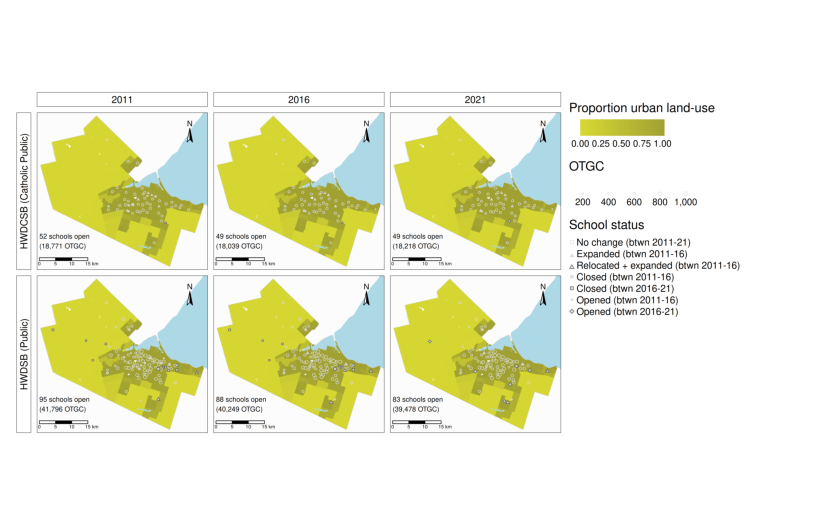
\includegraphics[width=1.2\textwidth,height=\textheight]{Manuscript_files/figure-pdf/fig-Fig2-1.pdf}

}

\caption{\label{fig-Fig2}The magnitude (top row) and rate per
residential unit (middle row) of elementary aged student population per
DA in 2011 and 2016. Bottom row: the proportion of low-income households
(prevelance of low-income after-tax, LIM-AT, measured by the 2011 and
2016 Canadian Census) with dependents under 18 years old shown. All
scales are represented in quartiles.}

\end{figure}%

\subsection{Estimated travel times and
emissions}\label{estimated-travel-times-and-emissions}

It is assumed that children can go to any elementary school, but there
is a preference for facilities that are more proximate. Based on this
assumption, the fourth source of data is information regarding the
mode-used and origin-destination locations of home-to-school trips from
the 2011 and 2016 TTS (Data Management Group 2018). The TTS is a travel
survey conducted in the Greater Golden Horseshoe Area in Ontario every
five years. With a target 5\% sampling rate, the survey is expanded to
be representative at the traffic analysis zone (TAZ) level of geography.
TAZ are spatial units created for the purpose of the TTS and pulled from
the R data package \{TTS2016R\} (Soukhov and Páez 2023); a few DAs
typically nest within each TAZ. The trip-level travel data extracted for
this paper represent 13,715 and 12,878 motorized trips (mode used
includes private car passenger, school bus, taxi, and transit) and 2,736
and 1,430 non-motorized trips (mode used includes walk and cycling) for
5 to 13 year olds from home-to-school in 2011 and 2016 respectively. The
travel times for motorized and non-motorized travel are estimated using
\{r5r\} (Pereira et al. 2021), which interfaces with the java-based R5
routing engine developed separately by Conveyal (Conveyal {[}2015{]}
2022). As travel times are not associated with the TTS, motorized and
non-motorized travel times are estimated for all TAZ centroids to all
TAZ centroids. We estimate motorized travel to be by car and
non-motorized travel to be by walk as those are the most used modes in
their respective categories. The travel times and the intensity of modal
home-to-school flows are visualised in Figure~\ref{fig-Fig3} along with
the boundaries of the TAZ and DAs. In Figure~\ref{fig-Fig3}, not all
TAZs capture an elementary school trip by both modes. For this reason,
the proportion of motorized modal share is aggregated at the community
level. Hamilton (Ancaster: 85\%-95\%, Dundas: 89\%-100\%, Flamborough:
91\%-97\%, Glanbrook: 92\%-95\%, Hamilton Central: 80\%-87\%, and Stoney
Creek: 82\%-88\%).

\begin{figure}[H]

\centering{

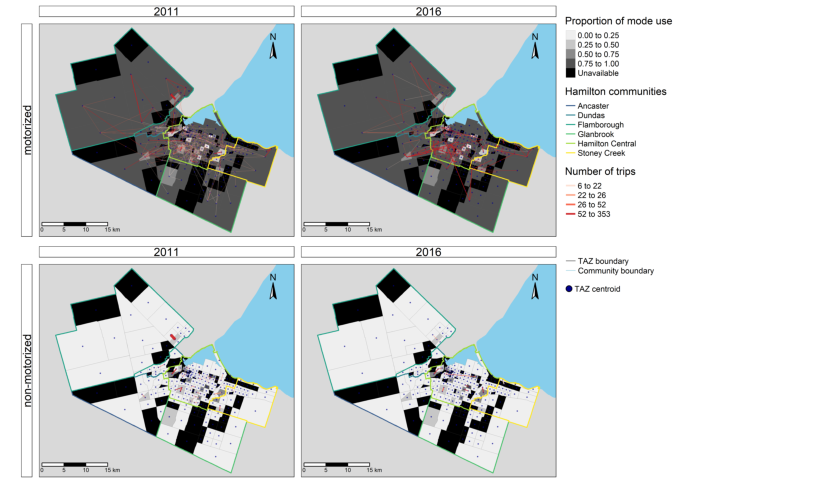
\includegraphics[width=1.2\textwidth,height=\textheight]{Manuscript_files/figure-pdf/fig-Fig3-1.pdf}

}

\caption{\label{fig-Fig3}The origin-destination flows from home-based
motorized and non-motorized school trips for students between 5-13 years
old as retrieved from TTS 2011 and 2016. Flows are mapped atop the
proportion of TAZ non/motorized modal share from the TTS 2011 and 2016,
DA boundaries, and Hamilton community boundaries.}

\end{figure}%

The fifth source of data consists of estimated travel time matrices from
all residential parcel locations to all elementary schools for both
motorized and non-motorized travel. The travel times are also estimated
using the \{r5r\} package (Pereira et al. 2021), with car mode and
walking representing motorized and non-motorized travel respectively.
For both motorized and non-motorized modes, the inputs assume a maximum
travel time threshold of 60 minutes and the free-flow OpenStreetMap road
network of Hamilton (retrieved using Geofabrik (Geofabrik 2022) and
manually edited to only include the network within Hamilton). Further,
only walking trips shorter than 27 min minutes were retained. This
travel time is approximately equivalent to 1.6 km which is the point
within-catchment students qualify for transport provided by the school
board (HWDSB 2019). Estimated trip-weighted motorized travel times are
on average 16.5 minutes in 2011 and 16.8 minutes in 2016 (summary
statistics for both years are approximately; min: 0.5, Q1: 11.0, Q2:
16.0, Q3: 21.0, max: 60.0). Estimated trip-weighted non-motorized travel
times are on average 18.0 minutes in 2011 and 18.1 minutes in 2016
(summary statistics for both years are approximately; min: 0.5, Q1:
13.0, Q2: 19.0, Q3: 24.0, max: 27.0).

These travel time matrices along with the origin-destination flows were
used to create modal trip length distribution (TLD) functions. Analysis
of the TLD is a useful technique to calibrate impedance functions as
they are a representation of the propensity of travel by trip length
(Horbachov and Svichynskyi 2018; Batista, Leclercq, and Geroliminis
2019). The empirical TLD is used to fit a density distribution using
maximum likelihood and moment matching techniques and the Nelder-Mead
and Brent methods for direct optimization available within the
\{fitdistrplus\} package (Delignette-Muller and Dutang 2015). Based on
goodness-of-fit criteria and diagnostics, the gamma and exponential
distributions were selected for the motorized and non-motorized modal
distributions respectively. The gamma distribution is defined by the
shape (\(\alpha\)) parameter of 1.939 (2011) and 2.046 (2016) and the
rate (\(\beta\)) of 0.233 (2011) and 0.236 (2016). The exponential
distribution is defined by the rate (\(\beta\)) parameter of 0.092
(2011) and 0.1 (2016). The TLDs for the motorized and non-motorized
trips are shown in Figure~\ref{fig-Fig4}. For reference, the gamma
distribution and the exponential distribution function are displayed in
Equations (\ref{eq:exp-dist}) and (\ref{eq:gamma-dist}) where \(x\) is
\(c_{ij}\):

\begin{equation}
\label{eq:exp-dist}
f(x) = \beta e ^{-\beta x}
\end{equation}

\begin{equation}
\label{eq:gamma-dist}
\begin{aligned}
f(x, \alpha, \beta) = \frac {x^{\alpha-1}e^{-\frac{x}{\beta}}}{ \beta^{\alpha}\Gamma(\alpha)} \quad \text{for } 0 \leq x \leq \infty \\
\Gamma(\alpha) =  \int_{0}^{\infty} x^{\alpha-1}e^{-x} \,dx
\end{aligned}
\end{equation}

\begin{figure}[H]

\centering{

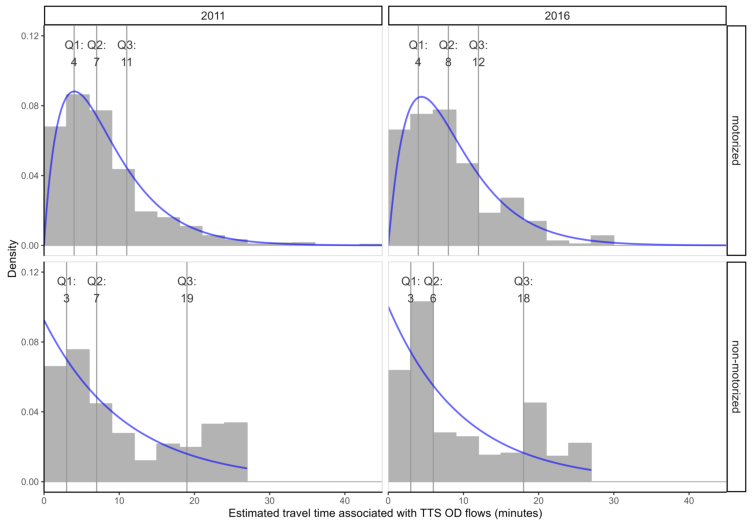
\includegraphics[width=1\textwidth,height=\textheight]{Manuscript_files/figure-pdf/fig-Fig4-1.pdf}

}

\caption{\label{fig-Fig4}Empirical (grey bars) and theoretical (blue
curves) motorized and non-motorized impedance functions. Motorized
theoretical impedance function is based on the gamma distribution
function and non-motorized on the expoential distribution function}

\end{figure}%

The sixth and final data source relates to motorized GHG estimations. It
assumed that all non-motorized trips produce no emissions and those that
are motorized take the average emission factor of 0.1 kg \(CO_{2}e\) per
minute travel. This emission factor is assumed based on an average speed
of 40 km/h, the 2,380 g \(CO_{2}e\) produced when 1 L of gasoline
(well-to-wheel) is combusted, and an internal combustion engine
passenger vehicle fuel efficiency of 7 g/100km as discussed in Soukhov
and Mohamed (2022).

\section{Methods: Multimodal spatial
availability}\label{methods-multimodal-spatial-availability}

Accessibility is defined as the ``potential for spatial interaction''.
It is classically presented as the gravity-based measure popularized by
Hansen (1959). It takes the following general multimodal formulation
(Equation (\ref{eq:multimodal-conventional-accessibility})):

\begin{equation}
\label{eq:multimodal-conventional-accessibility}
S_i^m = \sum_{j=1}^JO_j \cdot f^m(c_{ij}^m)
\end{equation}

\noindent where:

\begin{itemize}
\tightlist
\item
  \(m\) is a set of modes.
\item
  \(c_{ij}^m\) is a measure of the cost of moving between \(i\) and
  \(j\) for each \(m\).
\item
  \(f^m(\cdot)\) is an impedance function of \(c_{ij}^m\) for each
  \(m\); it can take the form of any monotonically decreasing function
  chosen based on positive or normative criteria (A. Páez, Scott, and
  Morency 2012).
\item
  \(i\) is a set of origin locations (\(i = 1,\cdots,N\)).
\item
  \(j\) is a set of destination locations (\(j = 1,\cdots,J\)).
\item
  \(O_j\) is the number of opportunities at location \(j\).
\item
  \(S\) is Hansen-type accessibility as weighted sum of opportunities.
\end{itemize}

As indicators of urban structure, Hansen-type measures are informative,
but the meaning of 10,000 accessible school-seats is harder to pin down:
how many opportunities must any single student have access to?
Furthermore, in scenario comparisons, the interpretation of the
percentage change in accessible school seats is unclear. The
interpretability of Hansen-type accessibility has been discussed in
numerous studies, including recently by Hu and Downs (2019), Kelobonye
et al. (2020), and in greater depth by Merlin and Hu (2017) along with
Soukhov et al. (2023) and Soukhov et al. (2024). The interpretation of
accessibility is suggested to depend on how many people demand the
opportunity, especially for exclusive opportunity-types like
schools-seats (i.e., one school-seat is for one student).

In this paper, we benefit from new developments in accessibility
research, particularly the multimodal spatial availability measure
(Soukhov et al. 2023; Soukhov et al. 2024). Spatial availability is a
singly-constrained accessibility measure that accounts for competition
by students using different modes for exclusive opportunities, such as
school seats. The measure's single constraint ensures that the marginals
at the destination are met and thus the number of estimated school seats
(opportunities) are preserved and allocated proportionally to the
mode-using student population. This proportional allocation of
opportunities yields an interpretable and meaningful measure of
opportunity access, particularly when comparing across modes, at the
spatial resolution of a residential parcel, and multiple time periods.
See Soukhov et al. (2024) for further discussion, multimodal spatial
availability \(V_{i}^m\) is defined as given by Equation
(\ref{eq:spatial-availability}).

\begin{equation}
\label{eq:spatial-availability}
V_{i}^{m} = \sum_{j=1}^J O_j\ F^{tm}_{ij}
\end{equation}

\noindent where:

\begin{itemize}
\tightlist
\item
  \(F^{tm}_{ij}\) is a balancing factor that depends on the population
  and cost of movement in the system as part of the gravity modelling
  framework and is captured in Equation (\ref{eq:balancing-factors}) for
  mode \(m\).
\item
  \(O_j\) is the number of opportunities at \(j\).
\item
  \(V_i^m\) is the number of spatially available opportunities from the
  perspective of \(i\) for mode \(m\).
\end{itemize}

\(F^{tm}_{ij}\) can be understood as the joint probability of allocating
opportunities, where \(F^{pm}_{i}\) is the population-based balancing
factor that grants a larger share of opportunities to larger \(m\)
population spatial units and \(F^{cm}_{ij}\) is the impedance-based
balancing factor that grants a larger share of the opportunities to less
\(m\)-travel costly centers. Together \(F^{tm}_{ij}\) ensures
proportional allocation such that opportunities \(O\) (like
school-seats) are preserved for the whole region (i.e.,
\(O = \sum_{j} O_j = \sum_{i} V_i = \sum_{m}\sum_{i} V_i^m\) ) and is
reflected in Equation (\ref{eq:balancing-factors}):

\begin{equation}
\label{eq:balancing-factors}
F^{tm}_{ij} = \frac{F^{pm}_{i} \cdot F^{cm}_{ij}}{\sum_{i} F^{pm}_{i} \cdot F^{cm}_{ij}}
\end{equation}

\noindent where:

\begin{itemize}
\tightlist
\item
  The factor for allocation by population for each \(m\) at each \(i\)
  is \(F^{pm}_{i} = \frac{P_{i}^m}{\sum_{m}\sum_{i} P_{i}^m}\)
\item
  The factor for allocation by travel cost for each \(m\) at each \(i\)
  and \(j\) is
  \(F^{cm}_{ij} = \frac{f^m(c^m_{ij})}{\sum_{m}\sum_{i} f^m(c^m_{ij})}\)
\end{itemize}

It should be noted that, when summed over all spatial units in the
region, the population-based allocation factors \(F^{pm}_{i}\) always
equal 1 (\(\sum_{m}\sum_{i} F^{pm}_{i}= 1\)), likewise for
impedance-based allocation factors \(F^{cm}_{i}\)
(\(\sum_{m}\sum_{i} F^{cm}_{ij} = 1\)).

Hansen-type accessibility is not designed to preserve the number of
opportunities in the region, it simply counts the intensity of
opportunities that those in a zone can potentially interact with
(weighted by the friction of distance). Also, as discussed in Soukhov et
al. (2023), popular competitive accessibility measures such as the 2SFCA
(Joseph and Bantock 1982; Weibull 1976; Shen 1998; Luo and Wang 2003)
are internally inconsistent, and the only way it preserves the number of
opportunities is if the effect of the impedance function is ignored when
expanding the values of opportunities per capita to obtain the total
number of opportunities. On the other hand, the proportional allocation
procedure associated with calculating multimodal spatial availability
\(V_i^m\) consistently returns a number of opportunities available to
populations by mode that matches the total number of opportunities in
the region when summed. By doing this consistently, it is possible to
define a measure of multimodal spatial availability per capita as
presented in Equation (\ref{eq:SA-per-capita}) for use as a benchmark to
compare against the regional opportunities per capita
(\(\frac{\sum_{j} O_j}{\sum_{i} P_i}\)).

\begin{equation}
\label{eq:SA-per-capita}
v_i^m = \frac{V_i^m}{P_i^m}
\end{equation}

This paper uses the multimodal spatial availability \(V_i^m\) and
spatial availability per student \(v_i^m\) measures to quantify
accessibility changes for the following reasons.

First, all residential parcels are associated to their respective census
DA, TTS TAZ, and community boundary based on spatial location
(aggregated by DA and shown as a per capita rate in the second row of
Figure~\ref{fig-Fig2}). Each parcel is assigned a number of `potential'
motorized and non-motorized student aged population (from DA) and modal
share (from TTS) to calculate a motorized and non-motorized population
balancing factor \(F_{i}^{pm}\). For each parcel, the following is
retained: the 2011 and 2016 census average elementary-aged student
population per parcel (Figure~\ref{fig-Fig2} second row) and the average
motorized and non-motorized share as informed by the TTS aggregated by
community (Figure~\ref{fig-Fig3}).

Second, the school capacity \(O_j\) is estimated and associated with
each school (Figure~\ref{fig-Fig1}). All residential locations are
assumed to be able to access all schools by non-motorized and/or
motorized mode. All origins (residential locations) can reach all
schools by motorized mode, but few residential locations can reach
schools within a 27 minute non-motorized trip.

Third, the motorized and non-motorized impedance-balancing factors
\(F_{ij}^{cm}\) are calculated using a mode-specific impedance function
(Figure~\ref{fig-Fig4}) based on the respective estimated travel times
for each origin (parcel) to school combination (OD flows retained from
the TTS). Using network estimated travel time sensitive to observed
parcel origin to school destination flows conceptually addresses the
aggregation error that could result from using less granular zonal units
to represent origin/destinations (Kane and Kim 2020; Kwan 1998; Hewko,
Smoyer-Tomic, and Hodgson 2002). Finally, outputs from all three stages
are joined together. \(F_{i}^{pm}\) joined with \(F_{ij}^{cm}\) yields
the total balancing factor \(F^{tm}_{ij}\) which serves to
proportionally allocate the school capacity \(O_j\) to each parcel. The
value is multimodal spatial availability \(V_i^m\) which can be
interpreted as the number of school-seats that are available to the
mode-using population at that parcel. \(V_i^m\) is then summed and
represented at the DA and community level along with the calculated
\(v_i^m\) for interpretation.

\section{Results}\label{results}

The motorized and non-motorized spatial availabilities of school seats
\(V_i^m\) for both 2011 and 2016 are presented in the top half of
Figure~\ref{fig-Fig5}. The sum of \(V_i^m\) values in a year for both
motorized and non-motorized population equals the city-wide OTGC (across
both public and catholic school boards) in that year. This is a result
of \(V_i^m\)'s proportional allocation mechanism, singly-constraining
opportunities through the proportion allocation balancing factors. In
this way, \(V_i^m\) results can be interpreted as a proportion of the
total OTGC in that year as the sum of \(V_i^m\) for both modes in a year
is equal to the total OTGC in that year. In Figure~\ref{fig-Fig5}, \(i\)
is a DA, so \(V_i^m\) is the sum of the school seat availability per
parcel in each DA. Each parcel is assigned a potential student
population based on the average rate of school-aged population per
residential parcel in that DA and the travel impedance weighted travel
time to all schools. The top four plots of Figure~\ref{fig-Fig5}
demonstrate different magnitudes in part due to significantly lower
non-motorized modal share (refer to Figure~\ref{fig-Fig3}), however it
is apparent that both mode using populations have higher spatial
availability when they are more proximate to schools. Hence, all DAs
have higher values within Hamilton Central and those more proximate to
schools in less-urban communities. Trends appear similar for both 2011
and 2016: this aligns with intuition, proximate populations using
motorized modes benefit from the ability to reach more distant
destinations than non-motorized modes.

When \(V_i^m\) is divided by the number of students by mode in that DA,
\(v_i^m\) is derived (bottom four plots in Figure~\ref{fig-Fig5}). The
\(v_i^m\) plots demonstrate different spatial distribution trends than
\(V_i^m\) plots. If our aim is to provide sufficient availability to
schools for both motorized and non-motorized populations (e.g., greater
than 1.0 \(v_i^m\) school-seat availability per student), this rate is
only achieved in the core of the city for motorized modes (greens and
yellows). Notably, this rate is only available to non-motorized
populations in DAs that are in less-densely populated rural areas that
are school proximate and very few pockets of Hamilton Central. The
majority of schools closed were within Hamilton Central, so
non-motorized populations in DAs within Hamilton Central were the most
negatively impacted by losses in availability while certain motorized
populations captured these losses as availability gains.

\begin{figure}[H]

\centering{

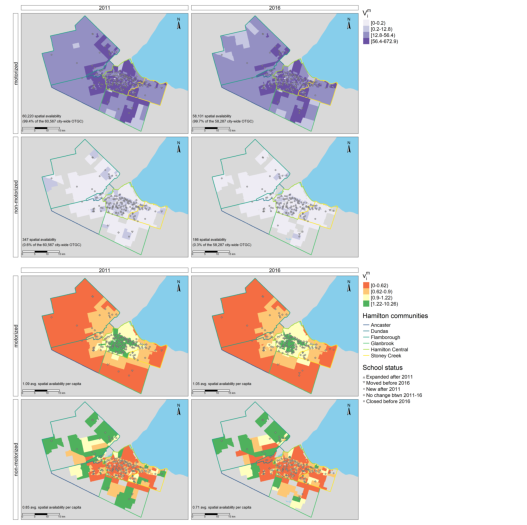
\includegraphics[width=1.2\textwidth,height=\textheight]{Manuscript_files/figure-pdf/fig-Fig5-1.pdf}

}

\caption{\label{fig-Fig5}Multimodal spatial availability (purples) and
spatial availability per mode-using student (diverging reds and greens)
aggregated at the DA level for 2011 and 2016. Scales are represented in
quartiles.}

\end{figure}%

To highlight this point, Figure~\ref{fig-Fig6} visualises the change in
school spatial availability between 2016 and 2011 for both mode where
\(i\) are 2016 DAs. Though the 2011 and 2016 DAs system are very similar
(see Figure~\ref{fig-Fig2} and Figure~\ref{fig-Fig3}), they are not
identical: 16 DAs changed in their spatial extent (i.e., added, removed,
changed boundaries). The proportional allocation mechanism of spatial
availability provides flexibility in aggregating parcel-level values at
whichever spatial unit is meaningful. For this case, the change in
\(V_i^m\) and \(v_i^m\) represented is the subtraction between the value
aggregated at 2016 DA for the 2016 and 2011 scenario.

\begin{figure}[H]

\centering{

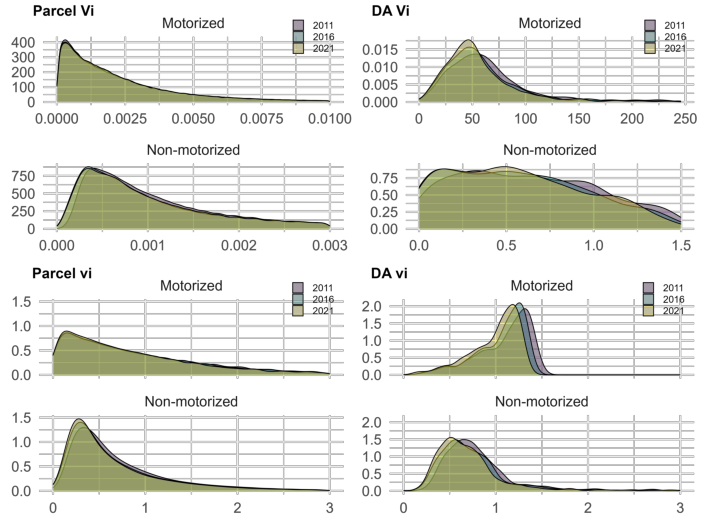
\includegraphics[width=1.2\textwidth,height=\textheight]{Manuscript_files/figure-pdf/fig-Fig6-1.pdf}

}

\caption{\label{fig-Fig6}Change in multimodal spatial availability and
spatial availability per mode-using student between 2016 and 2011.
Change is the subtraction of parcel-level results between 2016 and 2011
scenarios summed for each DA in the 2016 Canadian Census DA system.
Scales are represented in quartiles, with Q4 rounded to 0.}

\end{figure}%

From Figure~\ref{fig-Fig6} (top plots), it is apparent that decreases
(pinks and reds) in \(V_i^m\) appear across the city for both mode-using
populations. As the majority of closed schools are within the core of
the city: the more urban Hamilton Central and urban-areas of other
communities see a concentration of this decreased spatial availability
to school seats. Evidently, the number of OTGC in the city (equal to the
sum of \(V_i^m\)) decreased between the two years, so some sort of
decrease is to be expected. However, even when spatial availability is
divided by the mode-using population (which also decreased between the
years) \(v_i^m\) (bottom plots) continues to demonstrate decreases,
especially those locally proximate to closed schools.

This decrease follows different patterns depending on the mode.
\(v_i^{non-motorized}\) is most impacted for parcels within a 27 minute
walk travel time to schools that closed: these DAs demonstrate the most
dramatic decrease. Smaller-area DAs (in Hamilton-Central) and
larger-area DAs (in rural communities) proximate to closed schools
present Q1 decreases (red). For \(v_i^{motorized}\), the range offered
by motorized mode (estimated by shortest-path car travel times) is
city-wide, so since the majority of schools were centrally located, the
decrease is concentrated within the downtown core of Hamilton Central.
Some motorized-mode using populations in DAs do experience an increase
in \(V_i^m\) and \(v_i^m\): these DAs are often relatively proximate to
schools but more immediately outside walking range. Under competitive
and constrained calculations, these DAs benefit from the losses in
spatial availability that are predominately experienced by the
non-motorized populations within Hamilton Central.

The decrease in school seat spatial availability can be further
interpreted. How does potential non-motorized travel to school decrease?
How does the increase in potential motorized travel minutes impact GHG
emissions? Figure~\ref{fig-Fig7} visualises these related intermediates
for one-way home-to-school travel in a given day. The top plot of
Figure~\ref{fig-Fig7} demonstrates the sum of the change in
non-motorized minutes per 2016 DA. These travel time minutes are the
difference between the aggregated 2016 and 2011 scenarios for
non-motorized travel times multiplied by the proportion of
walking/cycling mode-use and rate of student population associated with
the parcels in each 2016 DA. It can be seen that Q1 decreases are
proximate to closed schools. Smaller decreases (and even a few
increases) are apparent in a range further from closed schools,
especially those also in proximity to the few opened/expanded schools.
Intuitively, these trends mirror what is shown within the
\(V^{non-motorized}\) landscape in Figure~\ref{fig-Fig6} (Pearson
correlation coefficient of 0.796) as travel time is an input into the
cost balancing factor \(F^{cm}_{ij}\). Similarly, the bottom plot
(Figure~\ref{fig-Fig7}) visualises the change in estimated emissions
from motorized travel minutes. The change in GHG emissions is also
highly correlated with \(V^{motorized}\) in Figure~\ref{fig-Fig6}
(Pearson correlation coefficient of 0.838) as it is also a product of
travel time.

\begin{figure}[H]

\centering{

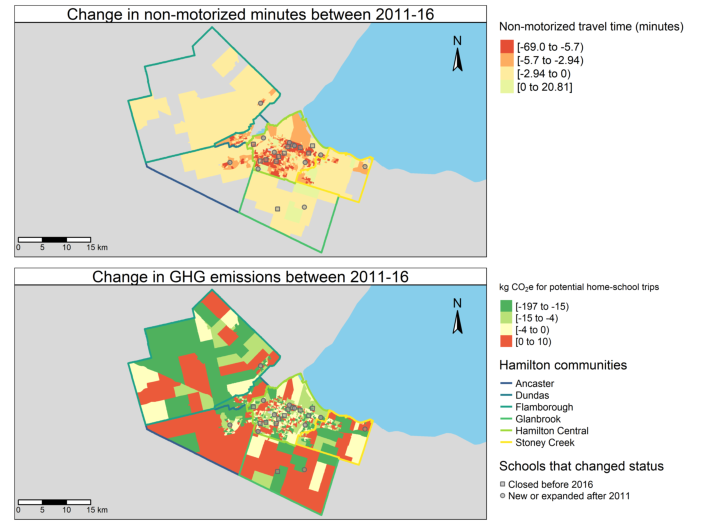
\includegraphics[width=0.9\textwidth,height=\textheight]{Manuscript_files/figure-pdf/fig-Fig7-1.pdf}

}

\caption{\label{fig-Fig7}Change in active travel time minutes (top plot)
and home-to-school GHG emissions (bottom plot) between 2011 and 2016
scenarios. Change is the subtraction of parcel-level results between
2016 and 2011 scenarios summed for each DA in the 2016 Canadian Census
DA system. Scales are represented in quartiles, with Q4 rounded to 0.}

\end{figure}%

Notably, the mode type of spatial availability loss is important. The
change in active travel minutes and GHG emissions highlights the
negative externalities of \emph{decreased} non-motorized spatial
availability. Normatively, our cities should be increasing spatial
availability for non-motorized mode users given the climate crisis. The
wave of school closures in Hamilton increased motorized spatial
availability and, hence, potential GHG emissions. The policy drastically
reduced non-motorized spatial availability, and this is seen in the
decrease in potential non-motorized travel minutes as well as increased
GHG emissions in rural areas that did benefit from motorized spatial
availability gains. The proportion of non-motorized mode use is low in
both 2011 and 2016, however, the closure of schools that are more
proximate to student-population density eliminates the potential of
those trips ever becoming active. And who is most impacted by the
reduction of non-motorized spatial availability? A summary of spatial
availability per Hamilton community and associated dimensions in 2016,
along with the percentage change between 2011 and 2016, is summarized in
Table~\ref{tbl-Tab1}.

\global\setlength{\Oldarrayrulewidth}{\arrayrulewidth}

\global\setlength{\Oldtabcolsep}{\tabcolsep}

\setlength{\tabcolsep}{2pt}

\renewcommand*{\arraystretch}{1.5}



\providecommand{\ascline}[3]{\noalign{\global\arrayrulewidth #1}\arrayrulecolor[HTML]{#2}\cline{#3}}

\begin{longtable}[c]{|p{0.47in}|p{0.40in}|p{0.29in}|p{0.38in}|p{0.34in}|p{0.40in}|p{0.29in}|p{0.38in}|p{0.29in}|p{0.40in}|p{0.29in}|p{0.38in}|p{0.29in}}

\caption{\label{tbl-Tab1}Spatial availability and associated dimensions
aggregated by communities}

\tabularnewline

\multicolumn{1}{>{\centering}p{\dimexpr 0.47in+0\tabcolsep}}{\textcolor[HTML]{000000}{\fontsize{6}{6}\selectfont{\textbf{}}}} & \multicolumn{2}{>{\centering}p{\dimexpr 0.7in+2\tabcolsep}}{\textcolor[HTML]{000000}{\fontsize{6}{6}\selectfont{\textbf{Hamilton\ C.}}}} & \multicolumn{2}{>{\centering}p{\dimexpr 0.72in+2\tabcolsep}}{\textcolor[HTML]{000000}{\fontsize{6}{6}\selectfont{\textbf{Dundas}}}} & \multicolumn{2}{>{\centering}p{\dimexpr 0.7in+2\tabcolsep}}{\textcolor[HTML]{000000}{\fontsize{6}{6}\selectfont{\textbf{Stoney\ Creek}}}} & \multicolumn{2}{>{\centering}p{\dimexpr 0.67in+2\tabcolsep}}{\textcolor[HTML]{000000}{\fontsize{6}{6}\selectfont{\textbf{Ancaster}}}} & \multicolumn{2}{>{\centering}p{\dimexpr 0.7in+2\tabcolsep}}{\textcolor[HTML]{000000}{\fontsize{6}{6}\selectfont{\textbf{Flamborough}}}} & \multicolumn{2}{>{\centering}p{\dimexpr 0.67in+2\tabcolsep}}{\textcolor[HTML]{000000}{\fontsize{6}{6}\selectfont{\textbf{Glanbrook}}}} \\





\multicolumn{1}{>{\centering}p{\dimexpr 0.47in+0\tabcolsep}}{\textcolor[HTML]{000000}{\fontsize{6}{6}\selectfont{\textbf{}}}} & \multicolumn{1}{>{\centering}p{\dimexpr 0.4in+0\tabcolsep}}{\textcolor[HTML]{000000}{\fontsize{6}{6}\selectfont{\textbf{}}}} & \multicolumn{1}{>{\centering}p{\dimexpr 0.29in+0\tabcolsep}}{\textcolor[HTML]{000000}{\fontsize{6}{6}\selectfont{\textbf{\%\ Δ}}}} & \multicolumn{1}{>{\centering}p{\dimexpr 0.38in+0\tabcolsep}}{\textcolor[HTML]{000000}{\fontsize{6}{6}\selectfont{\textbf{}}}} & \multicolumn{1}{>{\centering}p{\dimexpr 0.34in+0\tabcolsep}}{\textcolor[HTML]{000000}{\fontsize{6}{6}\selectfont{\textbf{\%\ Δ}}}} & \multicolumn{1}{>{\centering}p{\dimexpr 0.4in+0\tabcolsep}}{\textcolor[HTML]{000000}{\fontsize{6}{6}\selectfont{\textbf{}}}} & \multicolumn{1}{>{\centering}p{\dimexpr 0.29in+0\tabcolsep}}{\textcolor[HTML]{000000}{\fontsize{6}{6}\selectfont{\textbf{\%\ Δ}}}} & \multicolumn{1}{>{\centering}p{\dimexpr 0.38in+0\tabcolsep}}{\textcolor[HTML]{000000}{\fontsize{6}{6}\selectfont{\textbf{}}}} & \multicolumn{1}{>{\centering}p{\dimexpr 0.29in+0\tabcolsep}}{\textcolor[HTML]{000000}{\fontsize{6}{6}\selectfont{\textbf{\%\ Δ}}}} & \multicolumn{1}{>{\centering}p{\dimexpr 0.4in+0\tabcolsep}}{\textcolor[HTML]{000000}{\fontsize{6}{6}\selectfont{\textbf{}}}} & \multicolumn{1}{>{\centering}p{\dimexpr 0.29in+0\tabcolsep}}{\textcolor[HTML]{000000}{\fontsize{6}{6}\selectfont{\textbf{\%\ Δ}}}} & \multicolumn{1}{>{\centering}p{\dimexpr 0.38in+0\tabcolsep}}{\textcolor[HTML]{000000}{\fontsize{6}{6}\selectfont{\textbf{}}}} & \multicolumn{1}{>{\centering}p{\dimexpr 0.29in+0\tabcolsep}}{\textcolor[HTML]{000000}{\fontsize{6}{6}\selectfont{\textbf{\%\ Δ}}}} \\





\multicolumn{1}{>{\raggedright}p{\dimexpr 0.47in+0\tabcolsep}}{\textcolor[HTML]{000000}{\fontsize{6}{6}\selectfont{\textbf{LIM-AT}}}} & \multicolumn{1}{>{\raggedright}p{\dimexpr 0.4in+0\tabcolsep}}{\textcolor[HTML]{000000}{\fontsize{6}{6}\selectfont{27.0}}} & \multicolumn{1}{>{\raggedright}p{\dimexpr 0.29in+0\tabcolsep}}{\textcolor[HTML]{006400}{\fontsize{6}{6}\selectfont{14\%}}} & \multicolumn{1}{!{\color[HTML]{BEBEBE}\vrule width 1pt}>{\raggedright}p{\dimexpr 0.38in+0\tabcolsep}}{\textcolor[HTML]{000000}{\fontsize{6}{6}\selectfont{12.5}}} & \multicolumn{1}{>{\raggedright}p{\dimexpr 0.34in+0\tabcolsep}}{\textcolor[HTML]{006400}{\fontsize{6}{6}\selectfont{10\%}}} & \multicolumn{1}{!{\color[HTML]{BEBEBE}\vrule width 1pt}>{\raggedright}p{\dimexpr 0.4in+0\tabcolsep}}{\textcolor[HTML]{000000}{\fontsize{6}{6}\selectfont{11.6}}} & \multicolumn{1}{>{\raggedright}p{\dimexpr 0.29in+0\tabcolsep}}{\textcolor[HTML]{006400}{\fontsize{6}{6}\selectfont{10\%}}} & \multicolumn{1}{!{\color[HTML]{BEBEBE}\vrule width 1pt}>{\raggedright}p{\dimexpr 0.38in+0\tabcolsep}}{\textcolor[HTML]{000000}{\fontsize{6}{6}\selectfont{\ 8.9}}} & \multicolumn{1}{>{\raggedright}p{\dimexpr 0.29in+0\tabcolsep}}{\textcolor[HTML]{006400}{\fontsize{6}{6}\selectfont{24\%}}} & \multicolumn{1}{!{\color[HTML]{BEBEBE}\vrule width 1pt}>{\raggedright}p{\dimexpr 0.4in+0\tabcolsep}}{\textcolor[HTML]{000000}{\fontsize{6}{6}\selectfont{\ 7.6}}} & \multicolumn{1}{>{\raggedright}p{\dimexpr 0.29in+0\tabcolsep}}{\textcolor[HTML]{006400}{\fontsize{6}{6}\selectfont{4\%}}} & \multicolumn{1}{!{\color[HTML]{BEBEBE}\vrule width 1pt}>{\raggedright}p{\dimexpr 0.38in+0\tabcolsep}}{\textcolor[HTML]{000000}{\fontsize{6}{6}\selectfont{\ 7.5}}} & \multicolumn{1}{>{\raggedright}p{\dimexpr 0.29in+0\tabcolsep}}{\textcolor[HTML]{8B0000}{\fontsize{6}{6}\selectfont{-14\%}}} \\





\multicolumn{1}{>{\raggedright}p{\dimexpr 0.47in+0\tabcolsep}}{\textcolor[HTML]{000000}{\fontsize{6}{6}\selectfont{\textbf{Pop.}}}} & \multicolumn{1}{>{\raggedright}p{\dimexpr 0.4in+0\tabcolsep}}{\textcolor[HTML]{000000}{\fontsize{6}{6}\selectfont{33437.7}}} & \multicolumn{1}{>{\raggedright}p{\dimexpr 0.29in+0\tabcolsep}}{\textcolor[HTML]{8B0000}{\fontsize{6}{6}\selectfont{-4\%}}} & \multicolumn{1}{!{\color[HTML]{BEBEBE}\vrule width 1pt}>{\raggedright}p{\dimexpr 0.38in+0\tabcolsep}}{\textcolor[HTML]{000000}{\fontsize{6}{6}\selectfont{\ 2365.3}}} & \multicolumn{1}{>{\raggedright}p{\dimexpr 0.34in+0\tabcolsep}}{\textcolor[HTML]{8B0000}{\fontsize{6}{6}\selectfont{-8\%}}} & \multicolumn{1}{!{\color[HTML]{BEBEBE}\vrule width 1pt}>{\raggedright}p{\dimexpr 0.4in+0\tabcolsep}}{\textcolor[HTML]{000000}{\fontsize{6}{6}\selectfont{\ 8070.3}}} & \multicolumn{1}{>{\raggedright}p{\dimexpr 0.29in+0\tabcolsep}}{\textcolor[HTML]{006400}{\fontsize{6}{6}\selectfont{6\%}}} & \multicolumn{1}{!{\color[HTML]{BEBEBE}\vrule width 1pt}>{\raggedright}p{\dimexpr 0.38in+0\tabcolsep}}{\textcolor[HTML]{000000}{\fontsize{6}{6}\selectfont{\ 5387.5}}} & \multicolumn{1}{>{\raggedright}p{\dimexpr 0.29in+0\tabcolsep}}{\textcolor[HTML]{006400}{\fontsize{6}{6}\selectfont{12\%}}} & \multicolumn{1}{!{\color[HTML]{BEBEBE}\vrule width 1pt}>{\raggedright}p{\dimexpr 0.4in+0\tabcolsep}}{\textcolor[HTML]{000000}{\fontsize{6}{6}\selectfont{\ 5172.4}}} & \multicolumn{1}{>{\raggedright}p{\dimexpr 0.29in+0\tabcolsep}}{\textcolor[HTML]{8B0000}{\fontsize{6}{6}\selectfont{-4\%}}} & \multicolumn{1}{!{\color[HTML]{BEBEBE}\vrule width 1pt}>{\raggedright}p{\dimexpr 0.38in+0\tabcolsep}}{\textcolor[HTML]{000000}{\fontsize{6}{6}\selectfont{\ 4150.0}}} & \multicolumn{1}{>{\raggedright}p{\dimexpr 0.29in+0\tabcolsep}}{\textcolor[HTML]{006400}{\fontsize{6}{6}\selectfont{58\%}}} \\





\multicolumn{1}{>{\raggedright}p{\dimexpr 0.47in+0\tabcolsep}}{\textcolor[HTML]{000000}{\fontsize{6}{6}\selectfont{\textbf{OTGC}}}} & \multicolumn{1}{>{\raggedright}p{\dimexpr 0.4in+0\tabcolsep}}{\textcolor[HTML]{000000}{\fontsize{6}{6}\selectfont{36878.3}}} & \multicolumn{1}{>{\raggedright}p{\dimexpr 0.29in+0\tabcolsep}}{\textcolor[HTML]{8B0000}{\fontsize{6}{6}\selectfont{-8\%}}} & \multicolumn{1}{!{\color[HTML]{BEBEBE}\vrule width 1pt}>{\raggedright}p{\dimexpr 0.38in+0\tabcolsep}}{\textcolor[HTML]{000000}{\fontsize{6}{6}\selectfont{\ 2377.0}}} & \multicolumn{1}{>{\raggedright}p{\dimexpr 0.34in+0\tabcolsep}}{\textcolor[HTML]{000000}{\fontsize{6}{6}\selectfont{0\%}}} & \multicolumn{1}{!{\color[HTML]{BEBEBE}\vrule width 1pt}>{\raggedright}p{\dimexpr 0.4in+0\tabcolsep}}{\textcolor[HTML]{000000}{\fontsize{6}{6}\selectfont{\ 9387.8}}} & \multicolumn{1}{>{\raggedright}p{\dimexpr 0.29in+0\tabcolsep}}{\textcolor[HTML]{006400}{\fontsize{6}{6}\selectfont{4\%}}} & \multicolumn{1}{!{\color[HTML]{BEBEBE}\vrule width 1pt}>{\raggedright}p{\dimexpr 0.38in+0\tabcolsep}}{\textcolor[HTML]{000000}{\fontsize{6}{6}\selectfont{\ 3404.7}}} & \multicolumn{1}{>{\raggedright}p{\dimexpr 0.29in+0\tabcolsep}}{\textcolor[HTML]{006400}{\fontsize{6}{6}\selectfont{0\%}}} & \multicolumn{1}{!{\color[HTML]{BEBEBE}\vrule width 1pt}>{\raggedright}p{\dimexpr 0.4in+0\tabcolsep}}{\textcolor[HTML]{000000}{\fontsize{6}{6}\selectfont{\ 4638.2}}} & \multicolumn{1}{>{\raggedright}p{\dimexpr 0.29in+0\tabcolsep}}{\textcolor[HTML]{006400}{\fontsize{6}{6}\selectfont{2\%}}} & \multicolumn{1}{!{\color[HTML]{BEBEBE}\vrule width 1pt}>{\raggedright}p{\dimexpr 0.38in+0\tabcolsep}}{\textcolor[HTML]{000000}{\fontsize{6}{6}\selectfont{\ 1601.8}}} & \multicolumn{1}{>{\raggedright}p{\dimexpr 0.29in+0\tabcolsep}}{\textcolor[HTML]{006400}{\fontsize{6}{6}\selectfont{22\%}}} \\





\multicolumn{1}{>{\centering}p{\dimexpr 0.47in+0\tabcolsep}}{\textcolor[HTML]{000000}{\fontsize{6}{6}\selectfont{\textbf{}}}} & \multicolumn{12}{>{\centering}p{\dimexpr 4.15in+22\tabcolsep}}{\textcolor[HTML]{000000}{\fontsize{6}{6}\selectfont{\textbf{Motorized}}}} \\





\multicolumn{1}{>{\raggedright}p{\dimexpr 0.47in+0\tabcolsep}}{\textcolor[HTML]{000000}{\fontsize{6}{6}\selectfont{\textbf{V\ (mt)}}}} & \multicolumn{1}{>{\raggedright}p{\dimexpr 0.4in+0\tabcolsep}}{\textcolor[HTML]{000000}{\fontsize{6}{6}\selectfont{39626.9}}} & \multicolumn{1}{>{\raggedright}p{\dimexpr 0.29in+0\tabcolsep}}{\textcolor[HTML]{8B0000}{\fontsize{6}{6}\selectfont{-8\%}}} & \multicolumn{1}{!{\color[HTML]{BEBEBE}\vrule width 1pt}>{\raggedright}p{\dimexpr 0.38in+0\tabcolsep}}{\textcolor[HTML]{000000}{\fontsize{6}{6}\selectfont{\ 1817.7}}} & \multicolumn{1}{>{\raggedright}p{\dimexpr 0.34in+0\tabcolsep}}{\textcolor[HTML]{8B0000}{\fontsize{6}{6}\selectfont{-8\%}}} & \multicolumn{1}{!{\color[HTML]{BEBEBE}\vrule width 1pt}>{\raggedright}p{\dimexpr 0.4in+0\tabcolsep}}{\textcolor[HTML]{000000}{\fontsize{6}{6}\selectfont{\ 6656.8}}} & \multicolumn{1}{>{\raggedright}p{\dimexpr 0.29in+0\tabcolsep}}{\textcolor[HTML]{006400}{\fontsize{6}{6}\selectfont{6\%}}} & \multicolumn{1}{!{\color[HTML]{BEBEBE}\vrule width 1pt}>{\raggedright}p{\dimexpr 0.38in+0\tabcolsep}}{\textcolor[HTML]{000000}{\fontsize{6}{6}\selectfont{\ 4338.0}}} & \multicolumn{1}{>{\raggedright}p{\dimexpr 0.29in+0\tabcolsep}}{\textcolor[HTML]{006400}{\fontsize{6}{6}\selectfont{8\%}}} & \multicolumn{1}{!{\color[HTML]{BEBEBE}\vrule width 1pt}>{\raggedright}p{\dimexpr 0.4in+0\tabcolsep}}{\textcolor[HTML]{000000}{\fontsize{6}{6}\selectfont{\ 3290.3}}} & \multicolumn{1}{>{\raggedright}p{\dimexpr 0.29in+0\tabcolsep}}{\textcolor[HTML]{8B0000}{\fontsize{6}{6}\selectfont{-2\%}}} & \multicolumn{1}{!{\color[HTML]{BEBEBE}\vrule width 1pt}>{\raggedright}p{\dimexpr 0.38in+0\tabcolsep}}{\textcolor[HTML]{000000}{\fontsize{6}{6}\selectfont{\ 2371.7}}} & \multicolumn{1}{>{\raggedright}p{\dimexpr 0.29in+0\tabcolsep}}{\textcolor[HTML]{006400}{\fontsize{6}{6}\selectfont{58\%}}} \\





\multicolumn{1}{>{\raggedright}p{\dimexpr 0.47in+0\tabcolsep}}{\textcolor[HTML]{000000}{\fontsize{6}{6}\selectfont{\textbf{v\ (mt)}}}} & \multicolumn{1}{>{\raggedright}p{\dimexpr 0.4in+0\tabcolsep}}{\textcolor[HTML]{000000}{\fontsize{6}{6}\selectfont{1.2}}} & \multicolumn{1}{>{\raggedright}p{\dimexpr 0.29in+0\tabcolsep}}{\textcolor[HTML]{8B0000}{\fontsize{6}{6}\selectfont{-4\%}}} & \multicolumn{1}{!{\color[HTML]{BEBEBE}\vrule width 1pt}>{\raggedright}p{\dimexpr 0.38in+0\tabcolsep}}{\textcolor[HTML]{000000}{\fontsize{6}{6}\selectfont{0.8}}} & \multicolumn{1}{>{\raggedright}p{\dimexpr 0.34in+0\tabcolsep}}{\textcolor[HTML]{000000}{\fontsize{6}{6}\selectfont{0\%}}} & \multicolumn{1}{!{\color[HTML]{BEBEBE}\vrule width 1pt}>{\raggedright}p{\dimexpr 0.4in+0\tabcolsep}}{\textcolor[HTML]{000000}{\fontsize{6}{6}\selectfont{0.8}}} & \multicolumn{1}{>{\raggedright}p{\dimexpr 0.29in+0\tabcolsep}}{\textcolor[HTML]{000000}{\fontsize{6}{6}\selectfont{0\%}}} & \multicolumn{1}{!{\color[HTML]{BEBEBE}\vrule width 1pt}>{\raggedright}p{\dimexpr 0.38in+0\tabcolsep}}{\textcolor[HTML]{000000}{\fontsize{6}{6}\selectfont{0.8}}} & \multicolumn{1}{>{\raggedright}p{\dimexpr 0.29in+0\tabcolsep}}{\textcolor[HTML]{8B0000}{\fontsize{6}{6}\selectfont{-4\%}}} & \multicolumn{1}{!{\color[HTML]{BEBEBE}\vrule width 1pt}>{\raggedright}p{\dimexpr 0.4in+0\tabcolsep}}{\textcolor[HTML]{000000}{\fontsize{6}{6}\selectfont{0.6}}} & \multicolumn{1}{>{\raggedright}p{\dimexpr 0.29in+0\tabcolsep}}{\textcolor[HTML]{006400}{\fontsize{6}{6}\selectfont{2\%}}} & \multicolumn{1}{!{\color[HTML]{BEBEBE}\vrule width 1pt}>{\raggedright}p{\dimexpr 0.38in+0\tabcolsep}}{\textcolor[HTML]{000000}{\fontsize{6}{6}\selectfont{0.6}}} & \multicolumn{1}{>{\raggedright}p{\dimexpr 0.29in+0\tabcolsep}}{\textcolor[HTML]{000000}{\fontsize{6}{6}\selectfont{0\%}}} \\





\multicolumn{1}{>{\raggedright}p{\dimexpr 0.47in+0\tabcolsep}}{\textcolor[HTML]{000000}{\fontsize{6}{6}\selectfont{\textbf{GHG}}}} & \multicolumn{1}{>{\raggedright}p{\dimexpr 0.4in+0\tabcolsep}}{\textcolor[HTML]{000000}{\fontsize{6}{6}\selectfont{47788.1}}} & \multicolumn{1}{>{\raggedright}p{\dimexpr 0.29in+0\tabcolsep}}{\textcolor[HTML]{8B0000}{\fontsize{6}{6}\selectfont{-2\%}}} & \multicolumn{1}{!{\color[HTML]{BEBEBE}\vrule width 1pt}>{\raggedright}p{\dimexpr 0.38in+0\tabcolsep}}{\textcolor[HTML]{000000}{\fontsize{6}{6}\selectfont{\ 4851.7}}} & \multicolumn{1}{>{\raggedright}p{\dimexpr 0.34in+0\tabcolsep}}{\textcolor[HTML]{8B0000}{\fontsize{6}{6}\selectfont{-8\%}}} & \multicolumn{1}{!{\color[HTML]{BEBEBE}\vrule width 1pt}>{\raggedright}p{\dimexpr 0.4in+0\tabcolsep}}{\textcolor[HTML]{000000}{\fontsize{6}{6}\selectfont{15183.3}}} & \multicolumn{1}{>{\raggedright}p{\dimexpr 0.29in+0\tabcolsep}}{\textcolor[HTML]{006400}{\fontsize{6}{6}\selectfont{8\%}}} & \multicolumn{1}{!{\color[HTML]{BEBEBE}\vrule width 1pt}>{\raggedright}p{\dimexpr 0.38in+0\tabcolsep}}{\textcolor[HTML]{000000}{\fontsize{6}{6}\selectfont{\ 9470.9}}} & \multicolumn{1}{>{\raggedright}p{\dimexpr 0.29in+0\tabcolsep}}{\textcolor[HTML]{006400}{\fontsize{6}{6}\selectfont{14\%}}} & \multicolumn{1}{!{\color[HTML]{BEBEBE}\vrule width 1pt}>{\raggedright}p{\dimexpr 0.4in+0\tabcolsep}}{\textcolor[HTML]{000000}{\fontsize{6}{6}\selectfont{12839.1}}} & \multicolumn{1}{>{\raggedright}p{\dimexpr 0.29in+0\tabcolsep}}{\textcolor[HTML]{8B0000}{\fontsize{6}{6}\selectfont{-4\%}}} & \multicolumn{1}{!{\color[HTML]{BEBEBE}\vrule width 1pt}>{\raggedright}p{\dimexpr 0.38in+0\tabcolsep}}{\textcolor[HTML]{000000}{\fontsize{6}{6}\selectfont{\ 8798.4}}} & \multicolumn{1}{>{\raggedright}p{\dimexpr 0.29in+0\tabcolsep}}{\textcolor[HTML]{006400}{\fontsize{6}{6}\selectfont{60\%}}} \\





\multicolumn{1}{>{\raggedright}p{\dimexpr 0.47in+0\tabcolsep}}{\textcolor[HTML]{000000}{\fontsize{6}{6}\selectfont{\textbf{GHG/pop}}}} & \multicolumn{1}{>{\raggedright}p{\dimexpr 0.4in+0\tabcolsep}}{\textcolor[HTML]{000000}{\fontsize{6}{6}\selectfont{1.4}}} & \multicolumn{1}{>{\raggedright}p{\dimexpr 0.29in+0\tabcolsep}}{\textcolor[HTML]{006400}{\fontsize{6}{6}\selectfont{2\%}}} & \multicolumn{1}{!{\color[HTML]{BEBEBE}\vrule width 1pt}>{\raggedright}p{\dimexpr 0.38in+0\tabcolsep}}{\textcolor[HTML]{000000}{\fontsize{6}{6}\selectfont{2.1}}} & \multicolumn{1}{>{\raggedright}p{\dimexpr 0.34in+0\tabcolsep}}{\textcolor[HTML]{000000}{\fontsize{6}{6}\selectfont{0\%}}} & \multicolumn{1}{!{\color[HTML]{BEBEBE}\vrule width 1pt}>{\raggedright}p{\dimexpr 0.4in+0\tabcolsep}}{\textcolor[HTML]{000000}{\fontsize{6}{6}\selectfont{1.9}}} & \multicolumn{1}{>{\raggedright}p{\dimexpr 0.29in+0\tabcolsep}}{\textcolor[HTML]{000000}{\fontsize{6}{6}\selectfont{0\%}}} & \multicolumn{1}{!{\color[HTML]{BEBEBE}\vrule width 1pt}>{\raggedright}p{\dimexpr 0.38in+0\tabcolsep}}{\textcolor[HTML]{000000}{\fontsize{6}{6}\selectfont{1.8}}} & \multicolumn{1}{>{\raggedright}p{\dimexpr 0.29in+0\tabcolsep}}{\textcolor[HTML]{006400}{\fontsize{6}{6}\selectfont{2\%}}} & \multicolumn{1}{!{\color[HTML]{BEBEBE}\vrule width 1pt}>{\raggedright}p{\dimexpr 0.4in+0\tabcolsep}}{\textcolor[HTML]{000000}{\fontsize{6}{6}\selectfont{2.5}}} & \multicolumn{1}{>{\raggedright}p{\dimexpr 0.29in+0\tabcolsep}}{\textcolor[HTML]{000000}{\fontsize{6}{6}\selectfont{0\%}}} & \multicolumn{1}{!{\color[HTML]{BEBEBE}\vrule width 1pt}>{\raggedright}p{\dimexpr 0.38in+0\tabcolsep}}{\textcolor[HTML]{000000}{\fontsize{6}{6}\selectfont{2.1}}} & \multicolumn{1}{>{\raggedright}p{\dimexpr 0.29in+0\tabcolsep}}{\textcolor[HTML]{006400}{\fontsize{6}{6}\selectfont{2\%}}} \\





\multicolumn{1}{>{\centering}p{\dimexpr 0.47in+0\tabcolsep}}{\textcolor[HTML]{000000}{\fontsize{6}{6}\selectfont{\textbf{}}}} & \multicolumn{12}{>{\centering}p{\dimexpr 4.15in+22\tabcolsep}}{\textcolor[HTML]{000000}{\fontsize{6}{6}\selectfont{\textbf{Non-motorized}}}} \\





\multicolumn{1}{>{\raggedright}p{\dimexpr 0.47in+0\tabcolsep}}{\textcolor[HTML]{000000}{\fontsize{6}{6}\selectfont{\textbf{V\ (nmt)}}}} & \multicolumn{1}{>{\raggedright}p{\dimexpr 0.4in+0\tabcolsep}}{\textcolor[HTML]{000000}{\fontsize{6}{6}\selectfont{152.7}}} & \multicolumn{1}{>{\raggedright}p{\dimexpr 0.29in+0\tabcolsep}}{\textcolor[HTML]{8B0000}{\fontsize{6}{6}\selectfont{-44\%}}} & \multicolumn{1}{!{\color[HTML]{BEBEBE}\vrule width 1pt}>{\raggedright}p{\dimexpr 0.38in+0\tabcolsep}}{\textcolor[HTML]{000000}{\fontsize{6}{6}\selectfont{\ \ 0.0}}} & \multicolumn{1}{>{\raggedright}p{\dimexpr 0.34in+0\tabcolsep}}{\textcolor[HTML]{8B0000}{\fontsize{6}{6}\selectfont{-100\%}}} & \multicolumn{1}{!{\color[HTML]{BEBEBE}\vrule width 1pt}>{\raggedright}p{\dimexpr 0.4in+0\tabcolsep}}{\textcolor[HTML]{000000}{\fontsize{6}{6}\selectfont{\ 23.9}}} & \multicolumn{1}{>{\raggedright}p{\dimexpr 0.29in+0\tabcolsep}}{\textcolor[HTML]{8B0000}{\fontsize{6}{6}\selectfont{-42\%}}} & \multicolumn{1}{!{\color[HTML]{BEBEBE}\vrule width 1pt}>{\raggedright}p{\dimexpr 0.38in+0\tabcolsep}}{\textcolor[HTML]{000000}{\fontsize{6}{6}\selectfont{\ \ 4.0}}} & \multicolumn{1}{>{\raggedright}p{\dimexpr 0.29in+0\tabcolsep}}{\textcolor[HTML]{8B0000}{\fontsize{6}{6}\selectfont{-68\%}}} & \multicolumn{1}{!{\color[HTML]{BEBEBE}\vrule width 1pt}>{\raggedright}p{\dimexpr 0.4in+0\tabcolsep}}{\textcolor[HTML]{000000}{\fontsize{6}{6}\selectfont{\ \ 3.9}}} & \multicolumn{1}{>{\raggedright}p{\dimexpr 0.29in+0\tabcolsep}}{\textcolor[HTML]{8B0000}{\fontsize{6}{6}\selectfont{-64\%}}} & \multicolumn{1}{!{\color[HTML]{BEBEBE}\vrule width 1pt}>{\raggedright}p{\dimexpr 0.38in+0\tabcolsep}}{\textcolor[HTML]{000000}{\fontsize{6}{6}\selectfont{\ \ 1.9}}} & \multicolumn{1}{>{\raggedright}p{\dimexpr 0.29in+0\tabcolsep}}{\textcolor[HTML]{8B0000}{\fontsize{6}{6}\selectfont{-2\%}}} \\





\multicolumn{1}{>{\raggedright}p{\dimexpr 0.47in+0\tabcolsep}}{\textcolor[HTML]{000000}{\fontsize{6}{6}\selectfont{\textbf{v\ (nmt)}}}} & \multicolumn{1}{>{\raggedright}p{\dimexpr 0.4in+0\tabcolsep}}{\textcolor[HTML]{000000}{\fontsize{6}{6}\selectfont{0.6}}} & \multicolumn{1}{>{\raggedright}p{\dimexpr 0.29in+0\tabcolsep}}{\textcolor[HTML]{8B0000}{\fontsize{6}{6}\selectfont{-8\%}}} & \multicolumn{1}{!{\color[HTML]{BEBEBE}\vrule width 1pt}>{\raggedright}p{\dimexpr 0.38in+0\tabcolsep}}{\textcolor[HTML]{000000}{\fontsize{6}{6}\selectfont{0.0}}} & \multicolumn{1}{>{\raggedright}p{\dimexpr 0.34in+0\tabcolsep}}{\textcolor[HTML]{8B0000}{\fontsize{6}{6}\selectfont{-100\%}}} & \multicolumn{1}{!{\color[HTML]{BEBEBE}\vrule width 1pt}>{\raggedright}p{\dimexpr 0.4in+0\tabcolsep}}{\textcolor[HTML]{000000}{\fontsize{6}{6}\selectfont{0.7}}} & \multicolumn{1}{>{\raggedright}p{\dimexpr 0.29in+0\tabcolsep}}{\textcolor[HTML]{8B0000}{\fontsize{6}{6}\selectfont{-18\%}}} & \multicolumn{1}{!{\color[HTML]{BEBEBE}\vrule width 1pt}>{\raggedright}p{\dimexpr 0.38in+0\tabcolsep}}{\textcolor[HTML]{000000}{\fontsize{6}{6}\selectfont{0.7}}} & \multicolumn{1}{>{\raggedright}p{\dimexpr 0.29in+0\tabcolsep}}{\textcolor[HTML]{8B0000}{\fontsize{6}{6}\selectfont{-18\%}}} & \multicolumn{1}{!{\color[HTML]{BEBEBE}\vrule width 1pt}>{\raggedright}p{\dimexpr 0.4in+0\tabcolsep}}{\textcolor[HTML]{000000}{\fontsize{6}{6}\selectfont{1.7}}} & \multicolumn{1}{>{\raggedright}p{\dimexpr 0.29in+0\tabcolsep}}{\textcolor[HTML]{8B0000}{\fontsize{6}{6}\selectfont{-6\%}}} & \multicolumn{1}{!{\color[HTML]{BEBEBE}\vrule width 1pt}>{\raggedright}p{\dimexpr 0.38in+0\tabcolsep}}{\textcolor[HTML]{000000}{\fontsize{6}{6}\selectfont{1.4}}} & \multicolumn{1}{>{\raggedright}p{\dimexpr 0.29in+0\tabcolsep}}{\textcolor[HTML]{8B0000}{\fontsize{6}{6}\selectfont{-16\%}}} \\





\multicolumn{1}{>{\raggedright}p{\dimexpr 0.47in+0\tabcolsep}}{\textcolor[HTML]{000000}{\fontsize{6}{6}\selectfont{\textbf{tt}}}} & \multicolumn{1}{>{\raggedright}p{\dimexpr 0.4in+0\tabcolsep}}{\textcolor[HTML]{000000}{\fontsize{6}{6}\selectfont{4365.7}}} & \multicolumn{1}{>{\raggedright}p{\dimexpr 0.29in+0\tabcolsep}}{\textcolor[HTML]{8B0000}{\fontsize{6}{6}\selectfont{-38\%}}} & \multicolumn{1}{!{\color[HTML]{BEBEBE}\vrule width 1pt}>{\raggedright}p{\dimexpr 0.38in+0\tabcolsep}}{\textcolor[HTML]{000000}{\fontsize{6}{6}\selectfont{\ \ \ 0.0}}} & \multicolumn{1}{>{\raggedright}p{\dimexpr 0.34in+0\tabcolsep}}{\textcolor[HTML]{8B0000}{\fontsize{6}{6}\selectfont{-100\%}}} & \multicolumn{1}{!{\color[HTML]{BEBEBE}\vrule width 1pt}>{\raggedright}p{\dimexpr 0.4in+0\tabcolsep}}{\textcolor[HTML]{000000}{\fontsize{6}{6}\selectfont{\ 585.3}}} & \multicolumn{1}{>{\raggedright}p{\dimexpr 0.29in+0\tabcolsep}}{\textcolor[HTML]{8B0000}{\fontsize{6}{6}\selectfont{-28\%}}} & \multicolumn{1}{!{\color[HTML]{BEBEBE}\vrule width 1pt}>{\raggedright}p{\dimexpr 0.38in+0\tabcolsep}}{\textcolor[HTML]{000000}{\fontsize{6}{6}\selectfont{\ 103.3}}} & \multicolumn{1}{>{\raggedright}p{\dimexpr 0.29in+0\tabcolsep}}{\textcolor[HTML]{8B0000}{\fontsize{6}{6}\selectfont{-62\%}}} & \multicolumn{1}{!{\color[HTML]{BEBEBE}\vrule width 1pt}>{\raggedright}p{\dimexpr 0.4in+0\tabcolsep}}{\textcolor[HTML]{000000}{\fontsize{6}{6}\selectfont{\ \ 40.4}}} & \multicolumn{1}{>{\raggedright}p{\dimexpr 0.29in+0\tabcolsep}}{\textcolor[HTML]{8B0000}{\fontsize{6}{6}\selectfont{-62\%}}} & \multicolumn{1}{!{\color[HTML]{BEBEBE}\vrule width 1pt}>{\raggedright}p{\dimexpr 0.38in+0\tabcolsep}}{\textcolor[HTML]{000000}{\fontsize{6}{6}\selectfont{\ \ 22.5}}} & \multicolumn{1}{>{\raggedright}p{\dimexpr 0.29in+0\tabcolsep}}{\textcolor[HTML]{8B0000}{\fontsize{6}{6}\selectfont{12\%}}} \\





\multicolumn{1}{>{\raggedright}p{\dimexpr 0.47in+0\tabcolsep}}{\textcolor[HTML]{000000}{\fontsize{6}{6}\selectfont{\textbf{tt/pop}}}} & \multicolumn{1}{>{\raggedright}p{\dimexpr 0.4in+0\tabcolsep}}{\textcolor[HTML]{000000}{\fontsize{6}{6}\selectfont{18.2}}} & \multicolumn{1}{>{\raggedright}p{\dimexpr 0.29in+0\tabcolsep}}{\textcolor[HTML]{000000}{\fontsize{6}{6}\selectfont{0\%}}} & \multicolumn{1}{!{\color[HTML]{BEBEBE}\vrule width 1pt}>{\raggedright}p{\dimexpr 0.38in+0\tabcolsep}}{\textcolor[HTML]{000000}{\fontsize{6}{6}\selectfont{}}} & \multicolumn{1}{>{\raggedright}p{\dimexpr 0.34in+0\tabcolsep}}{\textcolor[HTML]{000000}{\fontsize{6}{6}\selectfont{}}} & \multicolumn{1}{!{\color[HTML]{BEBEBE}\vrule width 1pt}>{\raggedright}p{\dimexpr 0.4in+0\tabcolsep}}{\textcolor[HTML]{000000}{\fontsize{6}{6}\selectfont{17.8}}} & \multicolumn{1}{>{\raggedright}p{\dimexpr 0.29in+0\tabcolsep}}{\textcolor[HTML]{006400}{\fontsize{6}{6}\selectfont{2\%}}} & \multicolumn{1}{!{\color[HTML]{BEBEBE}\vrule width 1pt}>{\raggedright}p{\dimexpr 0.38in+0\tabcolsep}}{\textcolor[HTML]{000000}{\fontsize{6}{6}\selectfont{18.3}}} & \multicolumn{1}{>{\raggedright}p{\dimexpr 0.29in+0\tabcolsep}}{\textcolor[HTML]{006400}{\fontsize{6}{6}\selectfont{2\%}}} & \multicolumn{1}{!{\color[HTML]{BEBEBE}\vrule width 1pt}>{\raggedright}p{\dimexpr 0.4in+0\tabcolsep}}{\textcolor[HTML]{000000}{\fontsize{6}{6}\selectfont{17.9}}} & \multicolumn{1}{>{\raggedright}p{\dimexpr 0.29in+0\tabcolsep}}{\textcolor[HTML]{8B0000}{\fontsize{6}{6}\selectfont{-2\%}}} & \multicolumn{1}{!{\color[HTML]{BEBEBE}\vrule width 1pt}>{\raggedright}p{\dimexpr 0.38in+0\tabcolsep}}{\textcolor[HTML]{000000}{\fontsize{6}{6}\selectfont{16.4}}} & \multicolumn{1}{>{\raggedright}p{\dimexpr 0.29in+0\tabcolsep}}{\textcolor[HTML]{8B0000}{\fontsize{6}{6}\selectfont{-4\%}}} \\




\end{longtable}

\arrayrulecolor[HTML]{000000}

\global\setlength{\arrayrulewidth}{\Oldarrayrulewidth}

\global\setlength{\tabcolsep}{\Oldtabcolsep}

\renewcommand*{\arraystretch}{1}

Due to spatial availability's flexible proportional allocation mechanism
and this cases' calculation at the parcel level, results can also be
summarized by community (Table~\ref{tbl-Tab1}). The majority of schools
were closed in Hamilton Central. This community represents 60\% of the
5-14 year old population in 2016. Though the population between 2011 and
2016 decreased, the rate of school-seat spatial availability decreased
disproportionately more (population by -4\% and spatial availability by
-8\%). This disproportionate decrease is greatest in Hamilton Central
than any other community. This may have equity concerns as Hamilton
Central has the highest LIM-AT prevalence, with 27\% of households
LIM-AT in 2016, 3.7 times greater than Glanbrook, a community with the
lowest level of LIM-AT prevalence in the city. Between 2016 and 2011,
Hamilton Central had the lowest levels of emissions per student and saw
the highest per student increase in 2016. Hamilton Center had the
highest non-motorized trip potential, and it was reduced in part by the
school closure policies.

Conversely, communities with the lowest LIM-AT benefit the most, notably
in gains to motorized spatial availability. Glanbrook, Flamborough and
Ancaster have the lowest prevalence of LIM-AT of any Hamilton Community
and together account for 30\% of the 5-14 year old population in 2016.
These communities experienced a growth in student population (or only a
small decrease) and proportionally benefited from an increase in
motorized spatial availability.

Across the city, those who commute by non-motorized mode see the most
drastic lose in spatial availability. In all communities, spatial
availability decreases at greater levels than population. Notably in
Dundas (2nd highest LIM-AT), the only school in the community closed,
leaving the population in the community with no other option but to use
motorized modes. Glanbrook (lowest LIM-AT), which experienced a
relatively sharp increase in student population along with non-motorized
using population, suffered a lose in non-motorized spatial availability
despite seeing the highest increase in motorized spatial availability.
Overall, the gain in motorized spatial availability resulted in a
further erosion of non-motorized spatial availability. This erosion is
related to a lose in potential active home-to-school travel minutes
(3309.3 fewer minutes than in 2011, decreasing the potential active
travel time per (all mode using) student from 0.14 to 0.09 minutes), as
well as an increase in potential GHG emissions city-wide (3416 kg
\(CO_2e\) more emission than in 2011, increasing the kg \(CO_2e\) per
child rate for home-to-school trips from 1.64 to 1.68).

\section{Conclusion}\label{conclusion}

In this paper, we estimate the change in multimodal spatial availability
as a result of school consolidations/closures between the years of 2011
and 2016 in an empirical case study of Hamilton, a mid-size city
(\textasciitilde570,000 pop) in Ontario, Canada (Government of Canada
2022). The spatial availability and spatial availability per student are
calculated at the parcel level and aggregated at the Canadian Census DA
spatial unit and at the six Hamilton communities for comparison. Schools
closed and the number of school seats decreased so spatial availability
declined overall: we discuss where, for whom, and with what potential
impacts.

Overall, the closure of 7\% of elementary schools in Hamilton between
2011 and 2016 resulted in -4\% decline in school-seat availability
city-wide (2,280 fewer school-seats), but specifically a -46\% decline
in non-motorized spatial availability. Though non-motorized modal share
was low in both 2011 and 2016, the \emph{potential} for active transport
trips was significantly eroded as schools within a 27 minute walk
catchment were closed in the more densely populated and central areas of
the city. Further, the communities with the highest LIM-AT prevalence
were the most impacted: communities like Hamilton Central and Dundas saw
the most drastic loss in non-motorized spatial availability while
communities with lower LIM-AT prevalence saw gains in motorized spatial
availability (as a handful of rural schools opened). The motivation of
operational savings associated with public service consolidation for the
school boards did not account for the mobility-related burdens
\emph{certain} families are now saddled with.

In addition to spatial availability impacts, associated mobility
measures are assessed. City-wide, home-to-school non-motorized minutes
(for a one-way trip) reduced by 3,309 and GHG emissions associated with
motorized home-to-school travel increased by 3,416 kg \(CO_2e\). The
decision to consolidate schools, increase the length of motorized travel
and decrease the potential for non-motorized impacts will have daily
impacts on students and their families (Mandic et al. 2022; Pabayo et
al. 2012), the broader community (Pietrabissa 2023; Merrall, Higgins,
and Páez 2024; Bittencourt and Giannotti 2023) and the environment
(Pantelaki, Claudia Caspani, and Maggi 2024; Rong et al. 2022).

Like many other localities (J. Lee and Lubienski 2017; Autti and
Hyry-Beihammer 2014; Beuchert et al. 2018), Hamilton is not immune to
top-down operational efficiency assessments that determine if community
infrastructure is underutilized and closed. From the perspective of the
provincial government of Ontario, the school closures which occurred in
Hamilton resulted in operational savings-per-student. We demonstrate how
these decisions resulted in both families and students paying a price
through spatial availability, lost potential walk minutes, and increased
GHG emissions.

By quantifying the spatial availability, environmental, and
active-travel implications of school closure/consolidation policies in
Hamilton, our paper offers a methodology for spatial policy analysis
scenario. The presented methodology can be used by researchers and
decision-makers to plan and evaluate equitable and sustainable urban
planning policies from a spatial perspective. At the core of the method
is spatial availability (Soukhov et al. 2023; Soukhov et al. 2024), a
singly-constrained accessibility measure that can be calculated at the
finest spatial resolution (in our paper, parcel-level) and aggregated at
whichever spatial unit is most meaningful for interpretation. We urge
policy-makers to view the `spatial availability' of public resources
from a per-capita perspective, plan capacity and location of service
provision with the cost of travel (and associated implications such as
GHG emissions, active transportation mode, safety of active travel
modes, etc.) that sufficiently serves the target population. In this
work, we suggest and assume a benchmark of 1.0 school-seats per student
which accounts for sufficiency. Spatial availability can be used to
obtain this benchmark since the total number of opportunities (i.e.,
school capacity) is preserved in the region of analysis unlike
unconstrained forms of accessibility measurement e.g., Hansen-type
measure (Hansen 1959). As such, the assigned spatial availability can be
divided by population at each zone to yield an interpretable per capita
measurement.

Ultimately, this case study furnishes evidence that consolidation of
schools was particularly ill-timed: with the advent of the COVID-19
pandemic, the education system lacked the resiliency to accommodate
reduced classroom capacities and left parents who once lived within
active transportation distance to schools relying on motorized
transportation for their children. These top-down austerity measures
left the Hamilton local school system more vulnerable to the impacts of
COVID-19 by undervaluing the societal role of schools in neighbourhoods.
By identifying the impact of school consolidation policies in Ontario we
anticipate that researchers and decision-makers will have better
information to center the wellbeing of all residents, including
students, and the planet in urban planning policies.

As with all studies, our work is associated with limitations on how
results should be interpreted. The calculated spatial availability
assumes any residential parcel can have a student (at the DA rate of
students per residential unit) so all parcels are assigned a DA rate
weighted by how many residential units are contained within the parcel.
Each parcel can also visit any school, though travel times based on
observed origin-destination behaviour (from the TTS) are more likely
through the use of the empirical travel impedance functions. In this
way, the spatial availability demonstrates what \emph{potential
interaction} a student could have based on historic and average travel
behaviour and shortest network-path travel times if residing in point in
space. This representation is average, and by design obfuscates
considerations that could make non-average and shortest-path travel
unrealistic such as safety and built-environment concerns (C. Lee et al.
2021; Yumita et al. 2021) nor considers significant non-transportation
factors (Palm and Farber 2020). Further, this study does not consider
transit, school-bus, or cycling modes which have implications on how the
GHG emissions estimation can be interpreted. Transit and school bus
modes often taken more circuitous routes (Yumita et al. 2021) but pool
students thereby reducing emissions. Cycling reduces travel time over
the same walking distance at no extra emitted GHG. Lastly, this study
also ascribes a static emission factor to represent motorized travel
minutes based on an average diesel passenger car. In reality, GHG
emissions emitted per minute of driving varies extensively depending on
operating conditions and vehicle characteristics (Soukhov and Mohamed
2022). In these ways, the assumptions made are to illustrate
\emph{potential} and \emph{average} changes that resulted in a backdrop
of school consolidation/closures to illustrate accessibility-related
impacts for the city of Hamilton.

\pagebreak

\section{References}\label{references}

\phantomsection\label{refs}
\begin{CSLReferences}{1}{0}
\bibitem[\citeproctext]{ref-auditorgeneralofontarioAnnualReport20152015}
Auditor General of Ontario. 2015. {``Annual Report 2015.''} Office of
the Auditor General of Ontario.
\url{https://www.auditor.on.ca/en/content/annualreports/arreports/en15/2015AR_en_final.pdf}.

\bibitem[\citeproctext]{ref-Autti_Hyry-Beihammer_2014}
Autti, Outi, and Eeva Kaisa Hyry-Beihammer. 2014. {``School Closures in
Rural Finnish Communities.''} \emph{Journal of Research in Rural
Education} 29 (1): 1--17.

\bibitem[\citeproctext]{ref-batista_estimation_2019}
Batista, S. F. A., Ludovic Leclercq, and Nikolas Geroliminis. 2019.
{``Estimation of Regional Trip Length Distributions for the Calibration
of the Aggregated Network Traffic Models.''} \emph{Transportation
Research Part B: Methodological} 122 (April): 192--217.
\url{https://doi.org/10.1016/j.trb.2019.02.009}.

\bibitem[\citeproctext]{ref-von_Bergmann_Shkolnik_Jacobs_2021}
Bergmann, J von, D Shkolnik, and A Jacobs. 2021. \emph{Cancensus: R
Package to Access, Retrieve, and Work with Canadian Census Data and
Geography}.

\bibitem[\citeproctext]{ref-Beuchert_Humlum_Nielsen_Smith_2018}
Beuchert, Louise, Maria Knoth Humlum, Helena Skyt Nielsen, and Nina
Smith. 2018. {``The Short-Term Effects of School Consolidation on
Student Achievement: Evidence of Disruption?''} \emph{Economics of
Education Review} 65 (August): 31--47.
\url{https://doi.org/10.1016/j.econedurev.2018.05.004}.

\bibitem[\citeproctext]{ref-bierbaumMobilityJusticeLinking2021}
Bierbaum, Ariel H., Alex Karner, and Jesus M. Barajas. 2021. {``Toward
{Mobility Justice}: {Linking Transportation} and {Education Equity} in
the {Context} of {School Choice}.''} \emph{Journal of the American
Planning Association} 87 (2): 197--210.
\url{https://doi.org/10.1080/01944363.2020.1803104}.

\bibitem[\citeproctext]{ref-bittencourtEvaluatingAccessibilityAvailability2023}
Bittencourt, Tainá A., and Mariana Giannotti. 2023. {``Evaluating the
Accessibility and Availability of Public Services to Reduce Inequalities
in Everyday Mobility.''} \emph{Transportation Research Part A: Policy
and Practice} 177 (November): 103833.
\url{https://doi.org/10.1016/j.tra.2023.103833}.

\bibitem[\citeproctext]{ref-brunsdonOpeningPractice2021}
Brunsdon, Chris, and Alexis Comber. 2021. {``Opening Practice:
Supporting Reproducibility and Critical Spatial Data Science.''}
\emph{Journal of Geographical Systems} 23 (4): 477--96.
\url{https://doi.org/10.1007/s10109-020-00334-2}.

\bibitem[\citeproctext]{ref-butlerClosureRideau2019a}
Butler, Jesse K., Ruth G. Kane, and Fiona R. Cooligan. 2019. {``The
{Closure} of {Rideau High School}: {A Case Study} in the {Political
Economy} of {Urban Education} in {Ontario}.''} \emph{Canadian Journal of
Educational Administration and Policy}, no. 191.

\bibitem[\citeproctext]{ref-Statistics_Canada_2011}
Canada, Statistics. 2011. {``Census of Canda Census Profiles: Median
After-Tax Household Income, 5 to 9 Years, 10 to 14 Years, 15 to 19
Years, for Census Metroplian Areas and Dissimination Areas.''}

\bibitem[\citeproctext]{ref-Statistics_Canada_2016}
---------. 2016. {``Census of Canda Census Profiles: Median After-Tax
Household Income, 5 to 9 Years, 10 to 14 Years, 15 to 19 Years, for
Census Metroplian Areas and Dissimination Areas.''}

\bibitem[\citeproctext]{ref-Christiaanse_2020}
Christiaanse, Suzan. 2020. {``Rural Facility Decline: A Longitudinal
Accessibility Analysis Questioning the Focus of Dutch
Depopulation-Policy.''} \emph{Applied Geography} 121 (August): 102251.
\url{https://doi.org/10.1016/j.apgeog.2020.102251}.

\bibitem[\citeproctext]{ref-conveyalConveyalR5Routing2022}
Conveyal. (2015) 2022. {``Conveyal {R5 Routing Engine}.''} {Conveyal}.
\url{https://github.com/conveyal/r5}.

\bibitem[\citeproctext]{ref-craggsAxeCouldFall2012}
Craggs, Samantha. 2012. {``Axe Could Fall on More Hamilton Schools,
Projections Show.''} \emph{{CBC} News}, October.
\url{https://www.cbc.ca/news/canada/hamilton/headlines/axe-could-fall-on-more-hamilton-schools-projections-show-1.1183565}.

\bibitem[\citeproctext]{ref-craggsBoardEvaluatingFuture2013}
---------. 2013. {``Board Evaluating Future of 76 Public Elementary
Schools.''} \emph{{CBC} News}, February.
\url{https://www.cbc.ca/news/canada/hamilton/headlines/board-evaluating-future-of-76-public-elementary-schools-1.1347581}.

\bibitem[\citeproctext]{ref-Dai_Wang_Zhang_Liao_Liu_2019}
Dai, Te-qi, Liang Wang, Yu-chao Zhang, Cong Liao, and Zheng-bing Liu.
2019. {``The Cost of School Consolidation Policy: Implications from
Decomposing School Commuting Distances in Yanqing, Beijing.''}
\emph{Applied Spatial Analysis and Policy} 12 (2): 191--204.
\url{https://doi.org/10.1007/s12061-017-9238-2}.

\bibitem[\citeproctext]{ref-data_management_group_tts_2018}
Data Management Group. 2018. {``{TTS} - {Transportation} {Tomorrow}
{Survey} 2016.''}
\url{http://dmg.utoronto.ca/transportation-tomorrow-survey/tts-introduction}.

\bibitem[\citeproctext]{ref-fitdistrplus_2015}
Delignette-Muller, Marie Laure, and Christophe Dutang. 2015.
{``{fitdistrplus}: An {R} Package for Fitting Distributions.''}
\emph{Journal of Statistical Software} 64 (4): 1--34.
\url{https://www.jstatsoft.org/article/view/v064i04}.

\bibitem[\citeproctext]{ref-desjardinsFramingActive2024}
Desjardins, Elise, Jason Lam, Darcy Reynard, Damian Collins, E. Owen D.
Waygood, and Antonio Páez. 2024. {``Framing Active School Travel in
{Ontario}, or How Spinach Is Good for You.''} \emph{Transportation
Research Part A: Policy and Practice} 180 (February): 103953.
\url{https://doi.org/10.1016/j.tra.2024.103953}.

\bibitem[\citeproctext]{ref-faoOntarioSchoolBoards2023}
FAO. 2023. {``Ontario School Boards: Enrolment, Finances and Student
Outcomes.''} 978-1-4868-7600-6. Financial Accountability Office of
Ontario.
\url{https://www.fao-on.org/en/Blog/Publications/FA2207schoolboards}.

\bibitem[\citeproctext]{ref-geofabrikOntarioOpenStreetMapGeofabrik2022}
Geofabrik. 2022. {``Ontario {OpenStreetMap} - {Geofabrik Download
Server}.''} 2022.
\url{https://download.geofabrik.de/north-america/canada/ontario.html}.

\bibitem[\citeproctext]{ref-governmentofcanadaDictionaryCensusPopulation2017}
Government of Canada, Statistics Canada. 2017. {``Dictionary, Census of
Population, 2016 - Low-Income Measure, After Tax ({LIM}-{AT}).''} May 3,
2017.
\url{https://www12.statcan.gc.ca/census-recensement/2016/ref/dict/fam021-eng.cfm}.

\bibitem[\citeproctext]{ref-governmentofcanadaProfileTableCensus2022}
---------. 2022. {``Profile Table, Census Profile, 2021 Census of
Population - Hamilton, City (c) {[}Census Subdivision{]}, Ontario.''}
February 9, 2022.
\url{https://www12.statcan.gc.ca/census-recensement/2021/dp-pd/prof/index.cfm?Lang=E}.

\bibitem[\citeproctext]{ref-Hamilton_2014}
Hamilton. 2014. {``Map 5: Downtown Hamilton Buisness Improvement
Area.''} Hamilton.
\url{https://www.hamilton.ca/sites/default/files/media/browser/2014-11-27/downtown-hamilton-bia-map.pdf}.

\bibitem[\citeproctext]{ref-hansenHowAccessibilityShapes1959}
Hansen, Walter G. 1959. {``How {Accessibility Shapes Land Use}.''}
\emph{Journal of the American Institute of Planners} 25 (2): 73--76.
\url{https://doi.org/10.1080/01944365908978307}.

\bibitem[\citeproctext]{ref-hewkoMeasuringNeighbourhoodSpatial2002}
Hewko, Jared, Karen E Smoyer-Tomic, and M John Hodgson. 2002.
{``Measuring Neighbourhood Spatial Accessibility to Urban Amenities:
Does Aggregation Error Matter?''} \emph{Environment and Planning A:
Economy and Space} 34 (7): 1185--1206.
\url{https://doi.org/10.1068/a34171}.

\bibitem[\citeproctext]{ref-horbachov_theoretical_2018}
Horbachov, Peter, and Stanislav Svichynskyi. 2018. {``Theoretical
Substantiation of Trip Length Distribution for Home-Based Work Trips in
Urban Transit Systems.''} \emph{Journal of Transport and Land Use} 11
(1): 593--632. \url{https://www.jstor.org/stable/26622420}.

\bibitem[\citeproctext]{ref-hu_2019_measuring}
Hu, Yujie, and Joni Downs. 2019. {``Measuring and Visualizing
Place-Based Space-Time Job Accessibility.''} Journal Article.
\emph{Journal of Transport Geography} 74: 278--88.
\url{https://doi.org/10.1016/j.jtrangeo.2018.12.002}.

\bibitem[\citeproctext]{ref-hwdsbLongTermFacilities2013}
HWDSB. 2013. {``Long Term Facilities Master Plan - Accomodation Review
Schedule.''} Hamilton, Ontario: Hosted by {CBC}.
\url{https://www.documentcloud.org/documents/603032-hwdsb-schools-for-review}.

\bibitem[\citeproctext]{ref-HWDSB_2019}
HWDSB. 2019. {``Transportation: Policy No. 3.10.''}
\url{https://www.hamiltonschoolbus.ca/policies/hwdsb/HWDSB_Transportation_Policy.pdf}.

\bibitem[\citeproctext]{ref-irwinSchoolClosure2012}
Irwin, Bill, and Mark Seasons. 2012. {``School {Closure Decision-Making
Processes Problems} and {Prospects}.''} \emph{Canadian Journal of Urban
Research} 21 (2): 45--67.

\bibitem[\citeproctext]{ref-josephMeasuringPotentialPhysical1982}
Joseph, Alun E., and Peter R. Bantock. 1982. {``Measuring Potential
Physical Accessibility to General Practitioners in Rural Areas: A Method
and Case Study.''} \emph{Social Science \& Medicine} 16 (1): 85--90.
\url{https://doi.org/10.1016/0277-9536(82)90428-2}.

\bibitem[\citeproctext]{ref-kaneParcelsPointsProximity2020}
Kane, Kevin, and Young-An Kim. 2020. {``Parcels, Points, and Proximity:
Can Exhaustive Sources of Big Data Improve Measurement in Cities?''}
\emph{Environment and Planning B: Urban Analytics and City Science} 47
(4): 695--715. \url{https://doi.org/10.1177/2399808318797135}.

\bibitem[\citeproctext]{ref-kelobonye2020measuring}
Kelobonye, Keone, Heng Zhou, Gary McCarney, and Jianhong Xia. 2020.
{``Measuring the Accessibility and Spatial Equity of Urban Services
Under Competition Using the Cumulative Opportunities Measure.''} Journal
Article. \emph{Journal of Transport Geography} 85: 102706.
https://doi.org/\url{https://doi.org/10.1016/j.jtrangeo.2020.102706}.

\bibitem[\citeproctext]{ref-kleinhuisSeriousConcernsSchool2013}
Kleinhuis, Amanda. 2013. {``Serious Concerns about School Accommodation
Review Process - Raise the Hammer.''} 2013.
\url{https://www.raisethehammer.org/article/1979/serious_concerns_about_school_accommodation_review_process}.

\bibitem[\citeproctext]{ref-kwanSpaceTimeIntegralMeasures1998}
Kwan, Mei-Po. 1998. {``Space-Time and Integral Measures of Individual
Accessibility: A Comparative Analysis Using a Point-Based Framework.''}
\emph{Geographical Analysis} 30 (3): 191--216.
\url{https://doi.org/10.1111/j.1538-4632.1998.tb00396.x}.

\bibitem[\citeproctext]{ref-leeNeighborhoodEnvironmentsUtilitarian2021}
Lee, C, C Lee, OT Stewart, HA Carlos, A Adachi-Mejia, EM Berke, and MP
Doescher. 2021. {``Neighborhood Environments and Utilitarian Walking
Among Older Vs. Younger Rural Adults.''} \emph{{FRONTIERS} {IN} {PUBLIC}
{HEALTH}} 9 (June). \url{https://doi.org/10.3389/fpubh.2021.634751}.

\bibitem[\citeproctext]{ref-Lee_Lubienski_2017}
Lee, Jin, and Christopher Lubienski. 2017. {``The Impact of School
Closures on Equity of Access in Chicago.''} \emph{Education and Urban
Society} 49 (1): 53--80. \url{https://doi.org/10.1177/0013124516630601}.

\bibitem[\citeproctext]{ref-luoMeasuresSpatialAccessibility2003}
Luo, Wei, and Fahui Wang. 2003. {``Measures of {Spatial Accessibility}
to {Health Care} in a {GIS Environment}: {Synthesis} and a {Case Study}
in the {Chicago Region}.''} \emph{Environment and Planning B: Planning
and Design} 30 (6): 865--84. \url{https://doi.org/10.1068/b29120}.

\bibitem[\citeproctext]{ref-mackenzieBlueprintFixOntario2018}
Mackenzie, Hugh. 2018. {``A Blueprint to Fix Ontario's Education Funding
Formula.''} \emph{Canadian Centre for Policy Alternatives {\textbar}
Ontario}.
\url{https://policyalternatives.ca/sites/default/files/uploads/publications/Ontario\%20Office/2018/03/Course\%20Correction.pdf}.

\bibitem[\citeproctext]{ref-mandicAdolescentsPerceptionsWalking2022}
Mandic, Sandra, Enrique García Bengoechea, Debbie Hopkins, Kirsten
Coppell, and John C. Spence. 2022. {``Adolescents' Perceptions of
Walking and Cycling to School Differ Based on How Far They Live from
School.''} \emph{Journal of Transport \& Health} 24 (March): 101316.
\url{https://doi.org/10.1016/j.jth.2021.101316}.

\bibitem[\citeproctext]{ref-merlin2017competition}
Merlin, Louis A., and Lingqian Hu. 2017. {``Does Competition Matter in
Measures of Job Accessibility? Explaining Employment in Los Angeles.''}
Journal Article. \emph{Journal of Transport Geography} 64: 77--88.
\url{https://doi.org/10.1016/j.jtrangeo.2017.08.009}.

\bibitem[\citeproctext]{ref-Merrall_2021}
Merrall, John. 2021. {``The Effect of School Closures on House Prices in
Hamilton, Ontario.''} PhD thesis, McMaster University; School of Earth,
Environment,; Society.

\bibitem[\citeproctext]{ref-MerrallWhatsASchool2024}
Merrall, John, Christopher D. Higgins, and Antonio Páez. 2024. {``What's
a School Worth to a Neighborhood? {A} Spatial Hedonic Analysis of
Property Prices in the Context of Accommodation Reviews in Ontario.''}
\emph{Geographical Analysis} 56 (2): 217--43.
\url{https://doi.org/10.1111/gean.12377}.

\bibitem[\citeproctext]{ref-ministryofeducationPupilAccommodationReview2006}
Ministry of Education. 2006. {``Pupil Accommodation Review Guidelines -
Memo.''} Toronto: Business; Finance Divisio.
\url{https://efis.fma.csc.gov.on.ca/faab/Memos/B2006/B_12.pdf}.

\bibitem[\citeproctext]{ref-morencyHowMany2007}
Morency, C., M. Demers, and L. Lapierre. 2007. {``How Many Steps Do You
Have in Reserve? {Thoughts} and Measures about a Healthier Way to
Travel.''} \emph{Transportation Research Record} 2002: 1--6.
\url{https://doi.org/10.3141/2002-01}.

\bibitem[\citeproctext]{ref-morencyStepsReserve2009}
Morency, C., M. J. Roorda, and M. Demers. 2009. {``Steps in {Reserve
Comparing Latent Walk Trips} in {Toronto}, {Ontario}, and {Montreal},
{Quebec}, {Canada}.''} \emph{Transportation Research Record} 2140:
111--19. \url{https://doi.org/10.3141/2140-12}.

\bibitem[\citeproctext]{ref-ontarioSchoolFacilityInventory2017}
Ontario. 2017. {``School Facility Inventory System ({SFIS}) - Dataset -
Ontario Data Catalogue.''} February 2017.
\url{https://data.ontario.ca/dataset/school-facility-inventory-system-sfis}.

\bibitem[\citeproctext]{ref-OpenStreetMap_2021}
OpenStreetMap. 2021.

\bibitem[\citeproctext]{ref-pabayoImportanceActiveTransportation2012}
Pabayo, Roman, Katerina Maximova, John C. Spence, Kerry Vander Ploeg,
Biao Wu, and Paul J. Veugelers. 2012. {``The Importance of Active
Transportation to and from School for Daily Physical Activity Among
Children.''} \emph{Preventive Medicine} 55 (3): 196--200.
\url{https://doi.org/10.1016/j.ypmed.2012.06.008}.

\bibitem[\citeproctext]{ref-paezOpenSpatial2021c}
Páez, Antonio. 2021. {``Open Spatial Sciences: An Introduction.''}
\emph{Journal of Geographical Systems} 23 (4): 467--76.
\url{https://doi.org/10.1007/s10109-021-00364-4}.

\bibitem[\citeproctext]{ref-paez2012measuring}
Páez, A., D. M. Scott, and C. Morency. 2012. {``Measuring Accessibility:
Positive and Normative Implementations of Various Accessibility
Indicators.''} Journal Article. \emph{Journal of Transport Geography}
25: 141--53. \url{https://doi.org/10.1016/j.jtrangeo.2012.03.016}.

\bibitem[\citeproctext]{ref-palmRolePublicTransit2020}
Palm, Matthew, and Steven Farber. 2020. {``The Role of Public Transit in
School Choice and After-School Activity Participation Among Toronto High
School Students.''} \emph{Travel Behaviour and Society} 19 (April):
219--30. \url{https://doi.org/10.1016/j.tbs.2020.01.007}.

\bibitem[\citeproctext]{ref-pantelakiImpactHomeschoolCommuting2024}
Pantelaki, Evangelia, Anna Claudia Caspani, and Elena Maggi. 2024.
{``Impact of Home-School Commuting Mode Choice on Carbon Footprint and
Sustainable Transport Policy Scenarios.''} \emph{Case Studies on
Transport Policy} 15 (March): 101110.
\url{https://doi.org/10.1016/j.cstp.2023.101110}.

\bibitem[\citeproctext]{ref-Pereira2021r5r}
Pereira, Rafael H. M., Marcus Saraiva, Daniel Herszenhut, Carlos Kaue
Vieira Braga, and Matthew Wigginton Conway. 2021. {``R5r: Rapid
Realistic Routing on Multimodal Transport Networks with
r\textsuperscript{5} in r.''} \emph{Findings}, March.
\url{https://doi.org/10.32866/001c.21262}.

\bibitem[\citeproctext]{ref-pietrabissaSchoolAccessCity2023}
Pietrabissa, Giorgio. 2023. {``School Access and City Structure.''}
\url{https://giorgiopietrabissa.github.io/files/school_sorting.pdf}.

\bibitem[\citeproctext]{ref-rongReviewResearchLowcarbon2022}
Rong, Peijun, Mei-Po Kwan, Yaochen Qin, and Zhicheng Zheng. 2022. {``A
Review of Research on Low-Carbon School Trips and Their Implications for
Human-Environment Relationship.''} \emph{Journal of Transport Geography}
99 (February): 103306.
\url{https://doi.org/10.1016/j.jtrangeo.2022.103306}.

\bibitem[\citeproctext]{ref-Rosik_Pulawska-Obiedowska_Goliszek_2021}
Rosik, Piotr, Sabina Puławska-Obiedowska, and Sławomir Goliszek. 2021.
{``Public Transport Accessibility to Upper Secondary Schools Measured by
the Potential Quotient: The Case of Kraków.''} \emph{Moravian
Geographical Reports} 29 (1): 15--26.
\url{https://doi.org/10.2478/mgr-2021-0002}.

\bibitem[\citeproctext]{ref-sageman2022}
Sageman, Joseph. 2022. {``School Closures and Rural Population
Decline.''} \emph{Rural Sociology} 87 (3): 960--92.
\url{https://doi.org/10.1111/ruso.12437}.

\bibitem[\citeproctext]{ref-seasons2014ARCCatalogues2014}
Seasons, Mark. 2014a. {``2014 {ARC} Catalogues. 2014 English Public
{ARC} Inventory.''} 2014.
\url{https://uwaterloo.ca/school-closure-policy-research/research-findings/arc-data/2014-arc-catalogue}.

\bibitem[\citeproctext]{ref-seasonsSchoolClosurePolicy2014}
---------. 2014b. {``School Closure Policy {\textbar} School Closure
Policy Research.''} January 1, 2014.
\url{https://uwaterloo.ca/school-closure-policy-research/exploring-issue/school-closure-policy}.

\bibitem[\citeproctext]{ref-shenLocationCharacteristicsInnercity1998}
Shen, Q. 1998. {``Location Characteristics of Inner-City Neighborhoods
and Employment Accessibility of Low-Wage Workers.''} \emph{Environment
and Planning B: Planning and Design} 25 (3): 345--65.
\url{https://doi.org/10.1068/b250345}.

\bibitem[\citeproctext]{ref-soukhovOccupancyGHGEmissions2022}
Soukhov, Anastasia, and Moataz Mohamed. 2022. {``Occupancy and {GHG}
Emissions: Thresholds for Disruptive Transportation Modes and Emerging
Technologies.''} \emph{Transportation Research Part D: Transport and
Environment} 102 (January): 103127.
\url{https://doi.org/10.1016/j.trd.2021.103127}.

\bibitem[\citeproctext]{ref-soukhovTTS2016RDataSet2023}
Soukhov, Anastasia, and Antonio Páez. 2023. {``{TTS}2016R: A Data Set to
Study Population and Employment Patterns from the 2016 Transportation
Tomorrow Survey in the Greater Golden Horseshoe Area, Ontario,
Canada.''} \emph{Environment and Planning B: Urban Analytics and City
Science}, January, 23998083221146781.
\url{https://doi.org/10.1177/23998083221146781}.

\bibitem[\citeproctext]{ref-soukhovIntroducingSpatialAvailability2023}
Soukhov, Anastasia, Antonio Páez, Christopher D. Higgins, and Moataz
Mohamed. 2023. {``Introducing Spatial Availability, a Singly-Constrained
Measure of Competitive Accessibility \textbar{} {PLOS ONE}.''}
\emph{PLOS ONE}, 1--30.
https://doi.org/\href{https://\%20doi.org/10.1371/journal.pone.0278468}{https://
doi.org/10.1371/journal.pone.0278468}.

\bibitem[\citeproctext]{ref-soukhovMultimodalSpatialAvailability2024}
Soukhov, Anastasia, Javier Tarriño-Ortiz, Julio A. Soria-Lara, and
Antonio Páez. 2024. {``Multimodal Spatial Availability: A
Singly-Constrained Measure of Accessibility Considering Multiple
Modes.''} \emph{{PLOS} {ONE}} 19 (2): e0299077.
\url{https://doi.org/10.1371/journal.pone.0299077}.

\bibitem[\citeproctext]{ref-DMTI_Spatial_2015}
Spatial, DMTI. 2015. {``Building Footprints Region,''} September.
\url{http://geo.scholarsportal.info/\#r/details/_uri@=24}.

\bibitem[\citeproctext]{ref-Teranet_2009}
Teranet. 2009. {``Hamilton Parcel/Land Use Data.''} Dept. of Planning;
Economic Development.

\bibitem[\citeproctext]{ref-weibullAxiomaticApproachMeasurement1976}
Weibull, Jörgen W. 1976. {``An Axiomatic Approach to the Measurement of
Accessibility.''} \emph{Regional Science and Urban Economics} 6 (4):
357--79. \url{https://doi.org/10.1016/0166-0462(76)90031-4}.

\bibitem[\citeproctext]{ref-yumitaSchoolCommutingBarriers2021}
Yumita, FR, MZ Irawan, S Malkhamah, and MIH Kamal. 2021. {``School
Commuting: Barriers, Abilities and Strategies Toward Sustainable Public
Transport Systems in Yogyakarta, Indonesia.''} \emph{{SUSTAINABILITY}}
13 (16). \url{https://doi.org/10.3390/su13169372}.

\end{CSLReferences}

\pagebreak

\section{Appendix}\label{appendix}


% Table created by stargazer v.5.2.3 by Marek Hlavac, Social Policy Institute. E-mail: marek.hlavac at gmail.com
% Date and time: Thu, Apr 25, 2024 - 1:03:02 PM
\begin{table}[!htbp] \centering 
  \caption{Estimated on-the-ground capacity (OTGC) (units of school seats available per school) regression results for public and public-catholic school boards in Hamilton, Canada for years 2011 and 2016.} 
  \label{TabA1-OTGC} 
\begin{tabular}{@{\extracolsep{5pt}}lcc} 
\\[-1.8ex]\hline 
\hline \\[-1.8ex] 
 & \multicolumn{2}{c}{\textit{Dependent variable:}} \\ 
\\[-1.8ex] & \multicolumn{2}{c}{log(OTGC)} \\ 
\\[-1.8ex] & (Public) & (Catholic)\\ 
\hline \\[-1.8ex] 
 log(F) & 0.346$^{***}$ & 0.471$^{***}$ \\ 
  & (0.107) & (0.153) \\ 
  & & \\ 
 JrElem & 3.123$^{***}$ &  \\ 
  & (0.834) &  \\ 
  & & \\ 
 MidElem & 3.068$^{***}$ &  \\ 
  & (0.893) &  \\ 
  & & \\ 
 Elem & 3.752$^{***}$ &  2.333$^{*}$\\ 
  & (0.861) & (1.212) \\ 
  & & \\ 
 Sec & 4.094$^{***}$ &  2.936$^{**}$ \\ 
  & (0.978) & (1.398) \\ 
  & & \\ 
 urban.dist & $-$0.00003$^{***}$ & $-$0.00003$^{**}$ \\ 
  & (0.00001) & (0.00001) \\ 
  & & \\ 
\hline \\[-1.8ex] 
Observations & 42 & 42 \\ 
R$^{2}$ & 0.999 & 0.998 \\ 
Adjusted R$^{2}$ & 0.999 & 0.997 \\ 
Residual Std. Error & 0.212 (df = 36) & 0.331 (df = 38) \\ 
F Statistic & 6,189.428$^{***}$ (df = 6; 36) & 3,794.875$^{***}$ (df = 4; 38) \\ 
\hline 
\hline \\[-1.8ex] 
\textit{Note:}  & \multicolumn{2}{r}{$^{*}$p$<$0.1; $^{**}$p$<$0.05; $^{***}$p$<$0.01} \\ 
\end{tabular} 
\end{table} 




\end{document}
